% Options for packages loaded elsewhere
\PassOptionsToPackage{unicode}{hyperref}
\PassOptionsToPackage{hyphens}{url}
%
\documentclass[
]{article}
\usepackage{lmodern}
\usepackage{amssymb,amsmath}
\usepackage{ifxetex,ifluatex}
\ifnum 0\ifxetex 1\fi\ifluatex 1\fi=0 % if pdftex
  \usepackage[T1]{fontenc}
  \usepackage[utf8]{inputenc}
  \usepackage{textcomp} % provide euro and other symbols
\else % if luatex or xetex
  \usepackage{unicode-math}
  \defaultfontfeatures{Scale=MatchLowercase}
  \defaultfontfeatures[\rmfamily]{Ligatures=TeX,Scale=1}
\fi
% Use upquote if available, for straight quotes in verbatim environments
\IfFileExists{upquote.sty}{\usepackage{upquote}}{}
\IfFileExists{microtype.sty}{% use microtype if available
  \usepackage[]{microtype}
  \UseMicrotypeSet[protrusion]{basicmath} % disable protrusion for tt fonts
}{}
\makeatletter
\@ifundefined{KOMAClassName}{% if non-KOMA class
  \IfFileExists{parskip.sty}{%
    \usepackage{parskip}
  }{% else
    \setlength{\parindent}{0pt}
    \setlength{\parskip}{6pt plus 2pt minus 1pt}}
}{% if KOMA class
  \KOMAoptions{parskip=half}}
\makeatother
\usepackage{xcolor}
\IfFileExists{xurl.sty}{\usepackage{xurl}}{} % add URL line breaks if available
\IfFileExists{bookmark.sty}{\usepackage{bookmark}}{\usepackage{hyperref}}
\hypersetup{
  pdftitle={基于线性模型的锅炉冷壁温度曲线研究},
  pdfauthor={杜兴兴},
  hidelinks,
  pdfcreator={LaTeX via pandoc}}
\urlstyle{same} % disable monospaced font for URLs
\usepackage[left=3cm,right=3cm,top=3cm,bottom=3cm]{geometry}
\usepackage{longtable,booktabs}
% Correct order of tables after \paragraph or \subparagraph
\usepackage{etoolbox}
\makeatletter
\patchcmd\longtable{\par}{\if@noskipsec\mbox{}\fi\par}{}{}
\makeatother
% Allow footnotes in longtable head/foot
\IfFileExists{footnotehyper.sty}{\usepackage{footnotehyper}}{\usepackage{footnote}}
\makesavenoteenv{longtable}
\usepackage{graphicx}
\makeatletter
\def\maxwidth{\ifdim\Gin@nat@width>\linewidth\linewidth\else\Gin@nat@width\fi}
\def\maxheight{\ifdim\Gin@nat@height>\textheight\textheight\else\Gin@nat@height\fi}
\makeatother
% Scale images if necessary, so that they will not overflow the page
% margins by default, and it is still possible to overwrite the defaults
% using explicit options in \includegraphics[width, height, ...]{}
\setkeys{Gin}{width=\maxwidth,height=\maxheight,keepaspectratio}
% Set default figure placement to htbp
\makeatletter
\def\fps@figure{htbp}
\makeatother
\setlength{\emergencystretch}{3em} % prevent overfull lines
\providecommand{\tightlist}{%
  \setlength{\itemsep}{0pt}\setlength{\parskip}{0pt}}
\setcounter{secnumdepth}{5}
\usepackage[UTF8]{ctex}
\ifluatex
  \usepackage{selnolig}  % disable illegal ligatures
\fi

\title{基于线性模型的锅炉冷壁温度曲线研究}
\author{杜兴兴}
\date{2021-06-02}

\begin{document}
\maketitle

{
\setcounter{tocdepth}{2}
\tableofcontents
}

\hypertarget{ux6458ux8981}{%
\section{摘要}\label{ux6458ux8981}}

  在燃煤发电过程中,锅炉是一种重要的热能动力设备。锅炉的主要受热部分是水冷壁,其内部为流动的水用于吸收炉膛中高温燃烧产生的辐射热量,水受热蒸发产生高压蒸汽。影响水冷壁温度的因素有很多,本文旨在通过建立线性回归模型对水冷壁温度变化曲线进行分析研究。

  基于各个水冷壁管道的共5000组温度数据,从集中趋势、离中趋势及分布形态三个方面对数据进行描述。我们使用均值、标准差、最小值、最大值、波峰、趋势斜率等统计特征对10个水冷壁管道的温度时间序列数据进行分析,并辅以各管道温度变化的时序图和箱型图等综合分析管道温度的变化情况。在对各管道温度时间序列数据分析的基础上,基于题目给出的影响水冷壁温度的153个输入变量,首先对高维数据进行降维以便计算和可视化,采用弹性网约束的降维方式从中选取73个重要性变量;其次,在对比最小二乘回归和岭回归模型效果之后,选择效果更优的岭回归模型对10个水冷壁管道温度变化规律进行建模,并求解出各管道温度变化的线性回归方程。

  通过训练集和测试集拟合情况和模型拟合残差的分析,发现该模型拟合效果良好。在得到的岭回归模型基础上,通过绘制变量系数的重要性寻找重要影响变量,发现4角BC层二次风调节挡板位置反馈、1角A层二次风调节挡板位置反馈、A磨入口热一次风电调挡板位置、省煤器出口温度2、分离器出口汽温定值、A磨分离器风粉混合物温度2是关于水冷壁温度变化的重要影响变量,在实际操作过程中需要格外注意。

\textbf{关键词}:OLS、岭回归、水冷壁温度曲线

\newpage

\hypertarget{ux5f15ux8a00}{%
\section{引言}\label{ux5f15ux8a00}}

  在燃煤发电过程中,锅炉是一种重要的热能动力设备。它通过在炉膛中燃烧煤粉释放热量,将水加热成一定温度(或压力)的蒸汽,蒸汽再推动汽轮机旋转并驱动发电机发电。锅炉的主要受热部分是水冷壁,通常由数排钢管组成,分布于锅炉炉膛的四周,其内部为流动的水,用于吸收炉膛中高温燃烧产生的辐射热量,水受热蒸发产生高压蒸汽。

  在实际生产过程中,希望水冷壁的温度变化尽可能平稳,同时为保证安全,水冷壁温度不宜过高,否则有烧坏的风险。按照实际经验,操作人员给出的水冷壁温度超温报警线为445℃。影响水冷壁温度的因素有很多,包括锅炉负荷、蒸汽温度、蒸汽压力、燃料量、水煤比等。除了对水冷壁温度控制以外,识别出影响温度主要的操作变量对于工业生产和应用也是非常重要的。当然这个过程可以凭借专业的先验认知来确定,但为了可复用性,同时由于影响水冷壁温度的因素众多,因此需要建立一定的数学模型对其温度变化曲线进行分析和优化研究。

  本文对各个管道温度的均值进行拟合,然后将拟合模型应用到各个管道上。首先进行数据预处理,包括缺失值填补、异常值识别与处理、数据标准化、数据集划分。接下来进行降维处理后建立合适的统计模型。本文采用可接受性强、模型拟合效果较优的OLS回归与Ridge回归建立模型,并检验模型的是否有效,然后通过对比两个模型的拟合效果最终确定应用的模型。

\hypertarget{ux6570ux636eux4ecbux7ecd}{%
\section{数据介绍}\label{ux6570ux636eux4ecbux7ecd}}

\hypertarget{ux6570ux636eux6765ux6e90}{%
\subsection{数据来源}\label{ux6570ux636eux6765ux6e90}}

  数据来源于2021年长三角高校数学建模竞赛赛题数据。给出了10个具有代表性水冷壁管道的温度值,采样频率为15秒,共5000组数据;同时给出了影响水冷壁温度的153个输入变量的5000组数据,其中包括111个操作变量和42个状态变量。

  这里的操作变量,也常称作控制变量,是指在锅炉燃烧过程中,操作人员能够根据实际生产的需要而进行调节的量;而状态变量是用来描述锅炉燃烧系统运行状态的量,它的取值由相关检测设备采集得到,操作人员无法进行直接调节。

  由于原数据变量名较长且比较复杂,不便于编程实现和结果展示。因此,对所有输入变量的变量名进行统一编码。

  本文分析使用的软件为R语言
3.6版,统计分析主要用到的软件包为:tidyverse、Hmisc、glmnet、broom、MASS、ggplot2、dplyr、tidyr、readr,purrr、tibble、stringr、forcats。正文报告采用Rmarkdown中的knitr、pandoc包与LaTeX排版。

\hypertarget{ux6570ux636eux9884ux5904ux7406}{%
\subsection{数据预处理}\label{ux6570ux636eux9884ux5904ux7406}}

\hypertarget{ux7f3aux5931ux503cux586bux8865}{%
\subsubsection{缺失值填补}\label{ux7f3aux5931ux503cux586bux8865}}

  收集得到的数据某些字段值存在为空的情况,一般有三种处理方法:删除记录、数据填补、空值处理。填补缺失值方法有:人工填补、均数填补、中位数或众数填补、多重填补、使用最接近的样本值填补等。不同情况变量的缺失值本研究采用了不同的处理方式。当某一条观测数据缺失项大于总项的65\%时,由于缺失信息较大,故选择删除记录;考虑到不偏离原数据的总体分布,故在删除记录之后用列众数对缺失数据进行填补。处理之后还剩5000条观测数据,152个输入变量。

\hypertarget{ux6570ux636eux6807ux51c6ux5316}{%
\subsubsection{数据标准化}\label{ux6570ux636eux6807ux51c6ux5316}}

  不同的变量有不同的量纲,比如总给水流量、锅炉烟气含氧量、锅炉给水温度等,数值间的差别比较大,归一化就是为了消除变量之间量纲的影响。归一化就是将数据映射到某一固定区间,一般为(0,1)或(-1,1)。主要是为了数据处理方便提出来的,把有量纲表达式变成无量纲表达式。归一化公式:\(x^*=\frac{x-\bar{x}}{\sigma}\)。考虑到量纲不同问题,故本文对除结局变量外的所有变量均用归一化方法进行处理。处理之后共计还剩5000条有效观测数据,152个输入变量。

\hypertarget{ux5f02ux5e38ux503cux5904ux7406}{%
\subsubsection{异常值处理}\label{ux5f02ux5e38ux503cux5904ux7406}}

  库克距离用来判断强影响点是否为Y的异常值点:

\[D_i(M,c)=\frac{\left(\hat{\beta}(i)-\hat{\beta}\right)'M\left(\hat{\beta}(i)-\hat{\beta}\right)}{c}\]

  M是给定的正定矩阵,c是给定的常熟,当\(D_i{M,c}\)较大时,判定\((x'_i,y)\)为异常。一般认为当D\textless0.5时判断为非异常值点;当D\textgreater0.5时判断为异常值点。通过计算所以观测样本的Cook距离识别到如下6个异常值,见表1。

\begin{longtable}[]{@{}rrrrrrrrrrrr@{}}
\caption{Cook距离检测异常值样本结果表}\tabularnewline
\toprule
Time & Pipe0 & Pipe1 & Pipe2 & Pipe3 & Pipe4 & Pipe5 & Pipe6 & Pipe7 &
Pipe8 & Pipe9 & PipeMean\tabularnewline
\midrule
\endfirsthead
\toprule
Time & Pipe0 & Pipe1 & Pipe2 & Pipe3 & Pipe4 & Pipe5 & Pipe6 & Pipe7 &
Pipe8 & Pipe9 & PipeMean\tabularnewline
\midrule
\endhead
800 & 405.1 & 413.0 & 405.9 & 405.4 & 408.9 & 397.4 & 407.7 & 406.4 &
411.1 & 416.6 & 407.75\tabularnewline
963 & 407.6 & 415.0 & 407.0 & 406.1 & 408.5 & 396.8 & 408.5 & 405.9 &
413.1 & 418.6 & 408.71\tabularnewline
1221 & 387.3 & 403.0 & 406.1 & 405.0 & 402.6 & 391.1 & 392.9 & 384.7 &
399.9 & 406.6 & 397.92\tabularnewline
1222 & 386.5 & 401.8 & 405.0 & 404.0 & 401.7 & 389.7 & 392.5 & 384.4 &
399.8 & 406.0 & 397.14\tabularnewline
3990 & 375.3 & 397.8 & 397.0 & 391.8 & 394.5 & 381.7 & 386.3 & 378.7 &
420.3 & 436.0 & 395.94\tabularnewline
3991 & 376.1 & 397.7 & 396.9 & 391.8 & 394.6 & 382.0 & 386.5 & 379.5 &
420.2 & 434.9 & 396.02\tabularnewline
\bottomrule
\end{longtable}

  本文采用直接对异常值删除的方式进行处理,处理之后还剩4994条观测数据,152个输入变量。

\hypertarget{ux6570ux636eux96c6ux5212ux5206}{%
\subsubsection{数据集划分}\label{ux6570ux636eux96c6ux5212ux5206}}

  将上述处理之后数据按照采用时间的顺序,以7:3的比例划分为训练集和测试集。得到训练集共3491条观测,测试集共1503条观测。在描述分析过程中对全样本进行分析。在统计建模过程中,先在训练集上进行模型拟合,然后将模型应用至测试集进行模型效果评估。

\hypertarget{ux7edfux8ba1ux63cfux8ff0}{%
\section{统计描述}\label{ux7edfux8ba1ux63cfux8ff0}}

\hypertarget{ux57faux672cux7edfux8ba1ux7279ux5f81}{%
\subsection{基本统计特征}\label{ux57faux672cux7edfux8ba1ux7279ux5f81}}

  通过对11个(其中新增一列均值温度)水冷壁管道的数据分析,得到各个管道温度值的相关统计特征,见表2。从平均水平来看,各个管道的温度都在338℃~466℃的范围内波动。且平均温度最高的是管道10(424.92±18.70℃),最低是管道1(374.29±21.45℃),而管道9和管道10的温度均值在400℃以上,且最高温度值均高于超温报警线445℃,温度过高,有烧坏风险。整个水冷壁中出现的最高温度是在管道10中为465.40℃,最低温度出现在管道6为338.00℃。同时,各个管道温度的样本均值与样本中位数都非常匹配,没有发现任何异常现象。另外,表2中的最后两列分别为序列的波峰数和波谷数,通过识别序列的波峰波谷可以发现,整体上各个管道温度的变化波动都比较频繁,在4994个采样时间点上,出现了400次左右的波峰和波谷转折。

\begin{longtable}[]{@{}lrrrrrrrrr@{}}
\caption{各个管道温度基本统计特征表}\tabularnewline
\toprule
Pipes & Mean & Std & Max & Min & Q25 & Q50 & Q75 & PNum &
TNum\tabularnewline
\midrule
\endfirsthead
\toprule
Pipes & Mean & Std & Max & Min & Q25 & Q50 & Q75 & PNum &
TNum\tabularnewline
\midrule
\endhead
Pipe0 & 374.29 & 21.45 & 420.20 & 338.60 & 391.00 & 374.50 & 354.42 &
505 & 481\tabularnewline
Pipe1 & 397.90 & 16.86 & 426.60 & 356.80 & 411.20 & 401.30 & 389.40 &
398 & 404\tabularnewline
Pipe2 & 396.70 & 10.68 & 420.20 & 364.20 & 405.90 & 394.95 & 389.30 &
478 & 489\tabularnewline
Pipe3 & 387.59 & 16.38 & 420.90 & 350.60 & 404.10 & 387.10 & 373.70 &
579 & 533\tabularnewline
Pipe4 & 391.35 & 12.98 & 419.90 & 360.00 & 402.00 & 391.10 & 380.22 &
553 & 554\tabularnewline
Pipe5 & 376.83 & 16.66 & 409.50 & 338.00 & 391.90 & 377.10 & 362.00 &
436 & 438\tabularnewline
Pipe6 & 386.17 & 16.02 & 416.50 & 350.60 & 398.37 & 387.45 & 373.90 &
483 & 458\tabularnewline
Pipe7 & 378.67 & 17.21 & 421.30 & 351.20 & 390.90 & 376.70 & 362.80 &
952 & 963\tabularnewline
Pipe8 & 408.03 & 17.71 & 454.30 & 368.70 & 417.80 & 410.10 & 394.22 &
501 & 471\tabularnewline
Pipe9 & 424.92 & 18.70 & 465.40 & 378.80 & 441.80 & 423.20 & 412.42 &
406 & 386\tabularnewline
PipeMean & 392.25 & 13.72 & 417.68 & 361.42 & 403.83 & 394.81 & 379.28 &
398 & 407\tabularnewline
\bottomrule
\end{longtable}

\hypertarget{ux53efux89c6ux5316ux5206ux6790}{%
\subsection{可视化分析}\label{ux53efux89c6ux5316ux5206ux6790}}

  绘制各个管道温度的时序图,见图1。可以发现,10个水冷壁管道的温度变化范围基本在338℃~466℃以内。其温度变化均有一定的趋势,在取样点1000附近时,各个管道的温度都在平缓地上升,并达到最高值。随后各管道的温度在小范围内波动并以较快的速度下降到较低值,在取样点3500左右时又缓慢回升,最后趋于稳定温度。

  管道1~管道8的总体变化趋势较为相似,且其温度变化范围都在超温警戒线以内。而管道9和管道10均有超过警戒线445℃的取样时间段,且管道10在取样点3200后,多个时段温度超出445℃,出现明显的超温现象。

\begin{figure}

{\centering 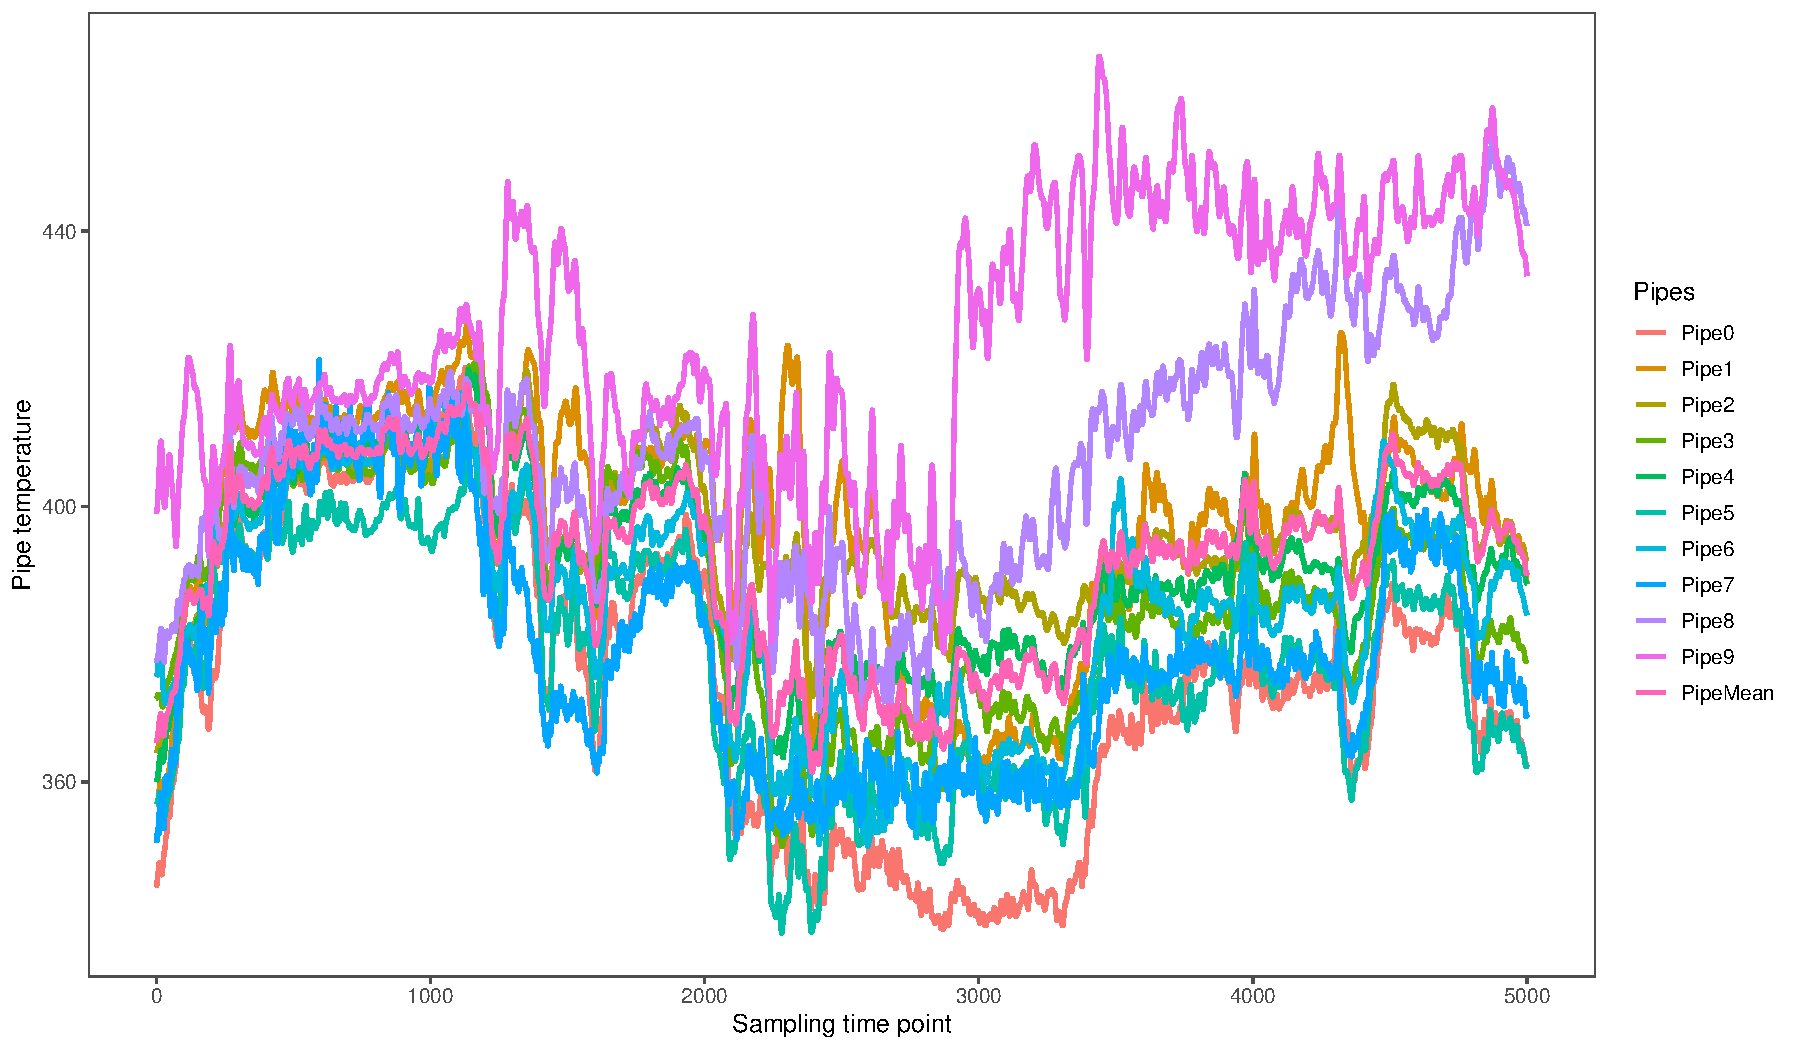
\includegraphics{TJRJCP_DuXingx_202105_files/figure-latex/unnamed-chunk-8-1} 

}

\caption{水冷壁管道温度的时序图}\label{fig:unnamed-chunk-8}
\end{figure}

  为了更好的描述各水冷壁管道温度数据的离散情况,我们使用箱型图进行进一步分析,见图2。箱型图最大的优点就是不受异常值的影响,能够以一种相对稳定的方式描述数据的离散分布情况。

\begin{figure}

{\centering 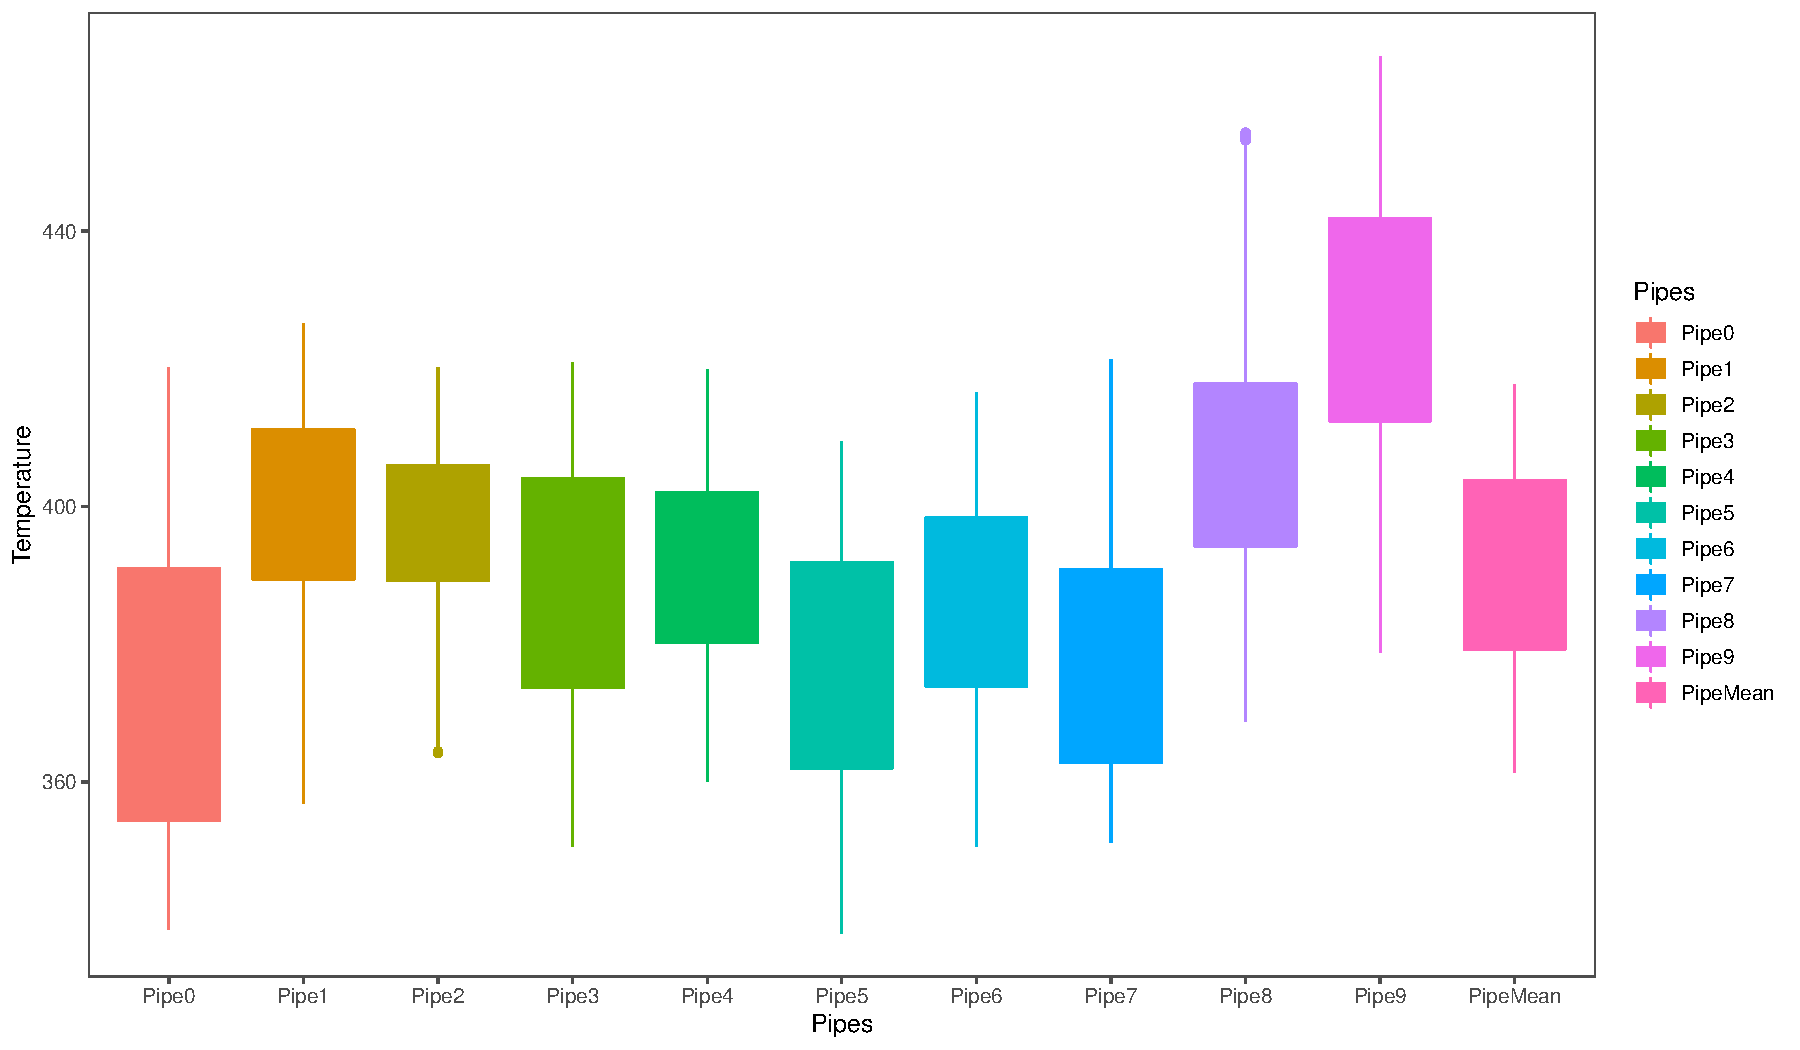
\includegraphics{TJRJCP_DuXingx_202105_files/figure-latex/unnamed-chunk-9-1} 

}

\caption{各个管道温度的箱线图}\label{fig:unnamed-chunk-9}
\end{figure}

  由图2可以分析得出,管道1的平均温度最低,管道10的平均温度最高。管道6的最高温度相较于其他管道最低,管道10的最高温度最大,且已超过警戒值445℃。管道3、9的温度值出现了离群点,存在异常值,而其他管道温度无异常值。管道平均温度处于中间水平,能够较好代表各个管道温度。

  由于管道平均温度能够较好代表各个管道温度,为了降低模型的冗余,故先在管道平均温度上进行分析,然后应用到各个单独的管道数据上。因此,绘制单独的管道平均温度进行观察,见图3。

\begin{figure}

{\centering 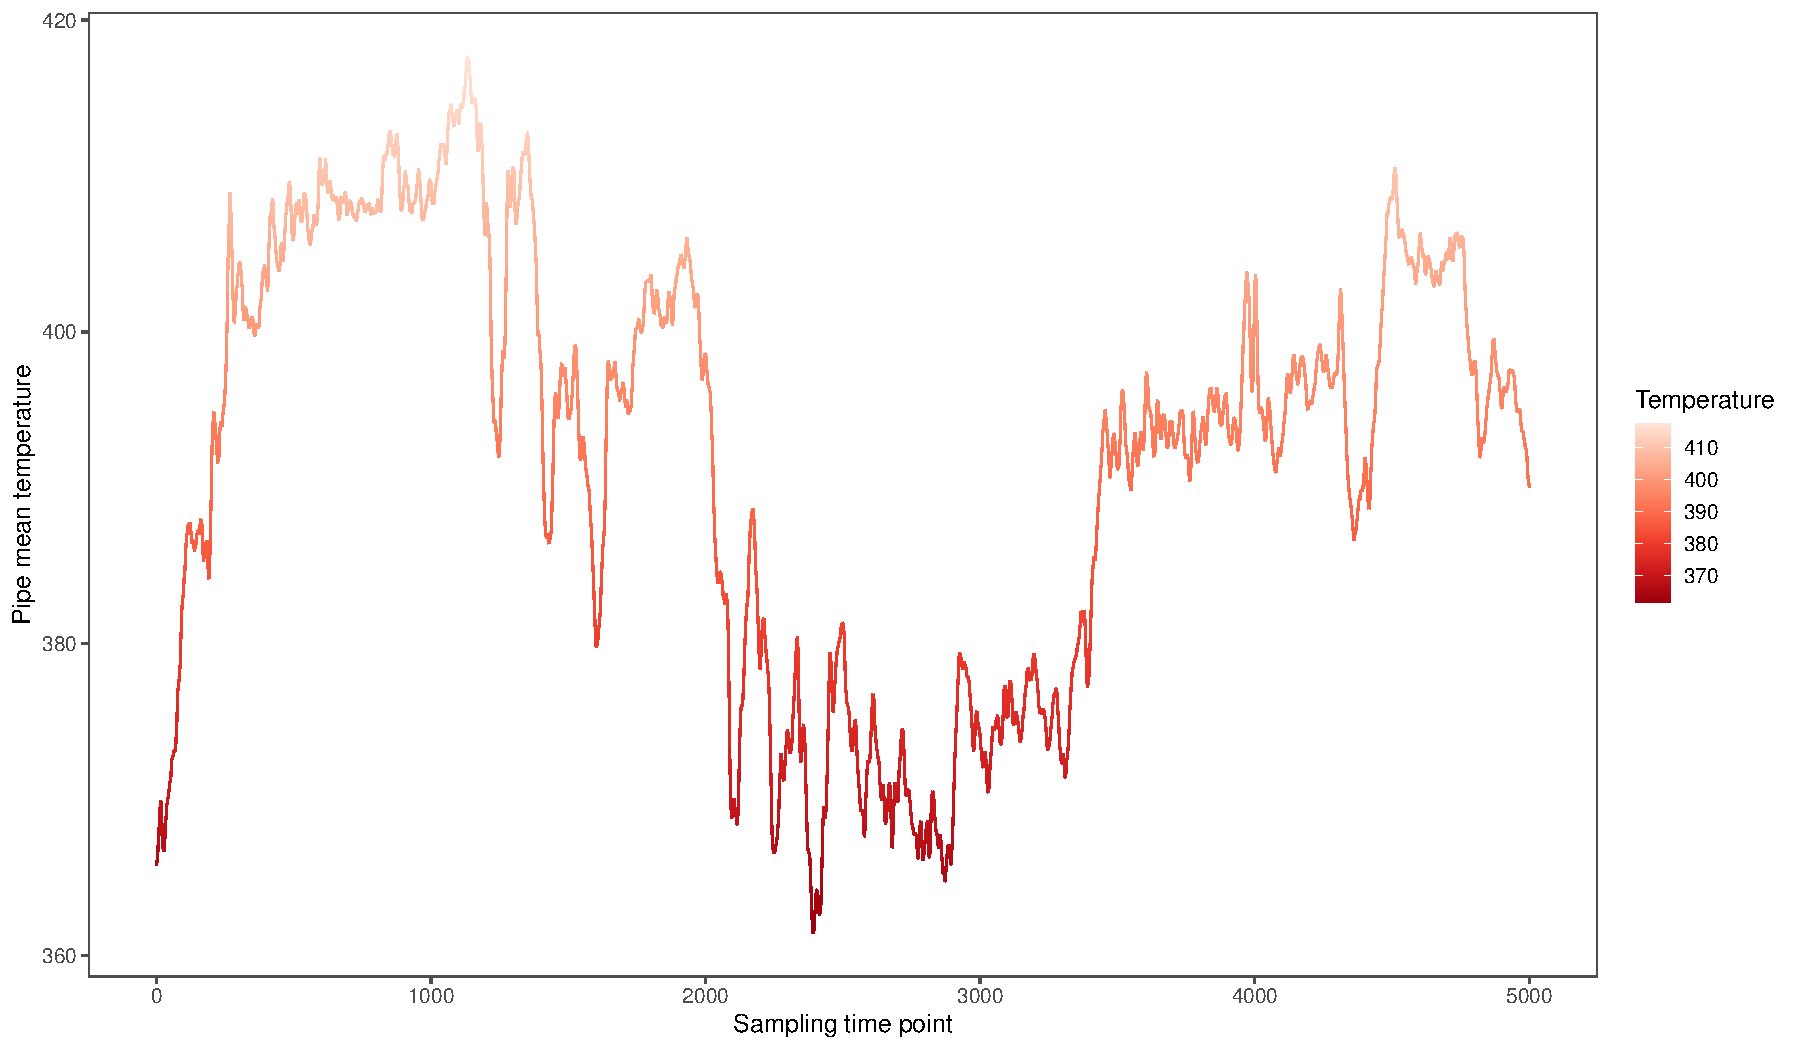
\includegraphics{TJRJCP_DuXingx_202105_files/figure-latex/unnamed-chunk-10-1} 

}

\caption{平均管道温度的时间序列图}\label{fig:unnamed-chunk-10}
\end{figure}

  管道平均温度的整体走势符合各个管道的温度走势,且存在同各个管道类似的时序特点,最高温度和最低温度都同上面所述的各个管道情况接近。

\hypertarget{ux76f8ux5173ux6027ux5206ux6790}{%
\subsection{相关性分析}\label{ux76f8ux5173ux6027ux5206ux6790}}

  通过计算各自变量与各个管道温度的相关系数,对得到的各个输入变量的相关系数绘制箱线图,见图
4。图中横轴表示不同的自变量,纵轴表示关于各个管道的相关系数的箱线图。

\begin{figure}

{\centering 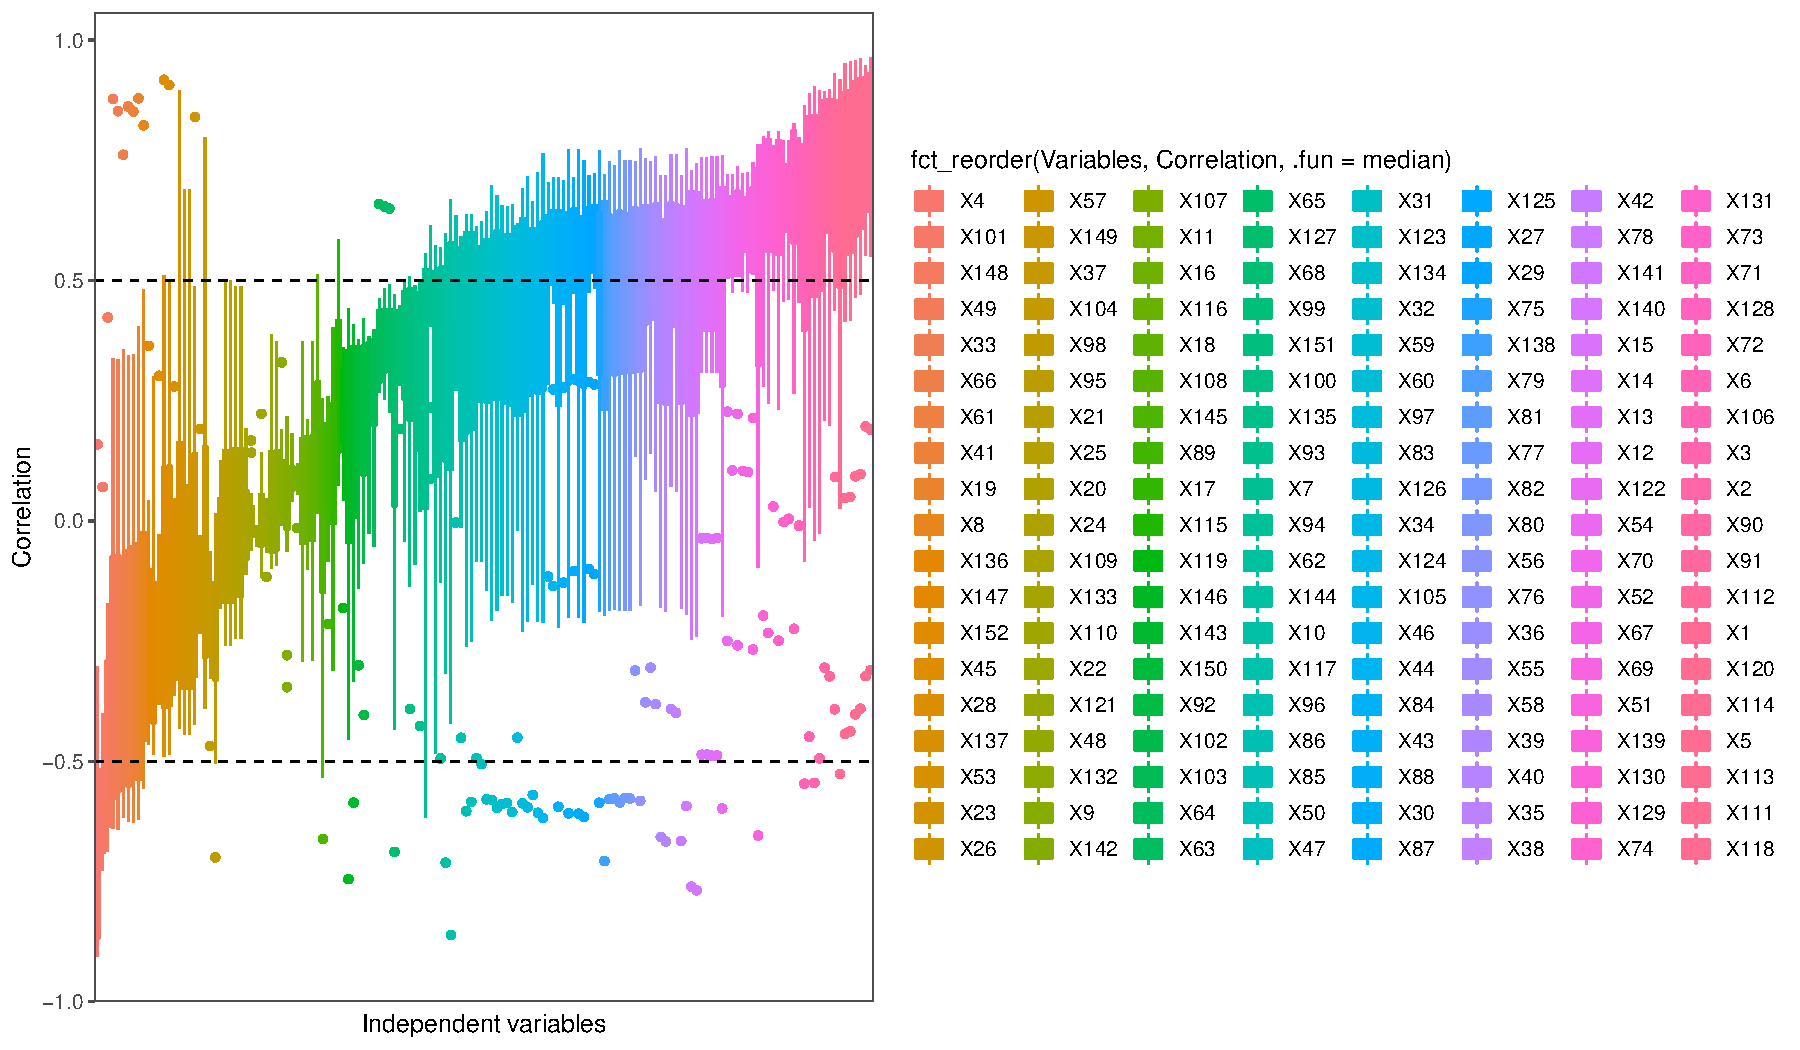
\includegraphics{TJRJCP_DuXingx_202105_files/figure-latex/unnamed-chunk-11-1} 

}

\caption{自变量与管道温度相关系数的箱线图}\label{fig:unnamed-chunk-11}
\end{figure}

 从图中可以发现,不同的变量对管道温度的相关性差异明显,存在多个高度正相关的输入变量,同时也存在一些高度负相关的输入变量。除此之外,还可以注意到在相关系数(-0.5,0.5)的范围内同样存在需要变量,从相关系数上来看,这些变量与因变量温度的相关性很低甚至无线性相关性。

  所以通过相关性分析知道输入变量中存在着大量的冗余变量。为了降低模型的复杂度,有降维的必要性,进而删除一些无关变量。

\hypertarget{ux5efaux6a21ux6a21ux578b}{%
\section{建模模型}\label{ux5efaux6a21ux6a21ux578b}}

\hypertarget{ux6570ux636eux964dux7ef4}{%
\subsection{数据降维}\label{ux6570ux636eux964dux7ef4}}

  常见的数据降维方法有很多种,例如主成分降维、Lasso降维、相关性降维等。本文通过对比不同参数下的弹性网约束估计降维,确定一个较优的降维参数。弹性网约束模型如下:

\[\hat{\beta}= arg min_{\beta}\left(\sum_{i}^n \left(y_i-\sum_{j=1}^p\beta_jx_{ij} \right)^2+\lambda_1\sum_{j=1}^p|p|+\lambda_2\sum_{j=1}^p\beta_j^2\right)\]

  从理论上可知,弹性网是综合了绝对约束和平方约束之后的模型,同时具有绝对约束估计和岭估计的特点。

\begin{itemize}
\item
  当\(\lambda=1\)时:弹性网约束估计就是岭回归;
\item
  当\(\lambda=0\)时:弹性网约束估计就是Lasso回归;
\end{itemize}

  本文通过设置不同的参数对比训练结果进而确定最终降维方法。设置的参数为\(\alpha=0\)(Ridge约束),0.25(弹性网约束),0.75(弹性网约束),1(Lasso约束)。得到如下的20折交叉验证的收敛图,见图5。从图中可知,横轴是对数\(\lambda\)值,纵轴是均方误差。按照此参数的设置,\(\alpha=0\)不会进行变量降维,\(\alpha=0.25\)保留的
变量个数为99个,\(\alpha=0.75\)保留的变量个数为99个,\(\alpha=0.75\)保留的变量个数为108个,\(\alpha=1\)保留的变量个数为88个,且四种参数设置下均方误差都接近0。

\begin{figure}

{\centering 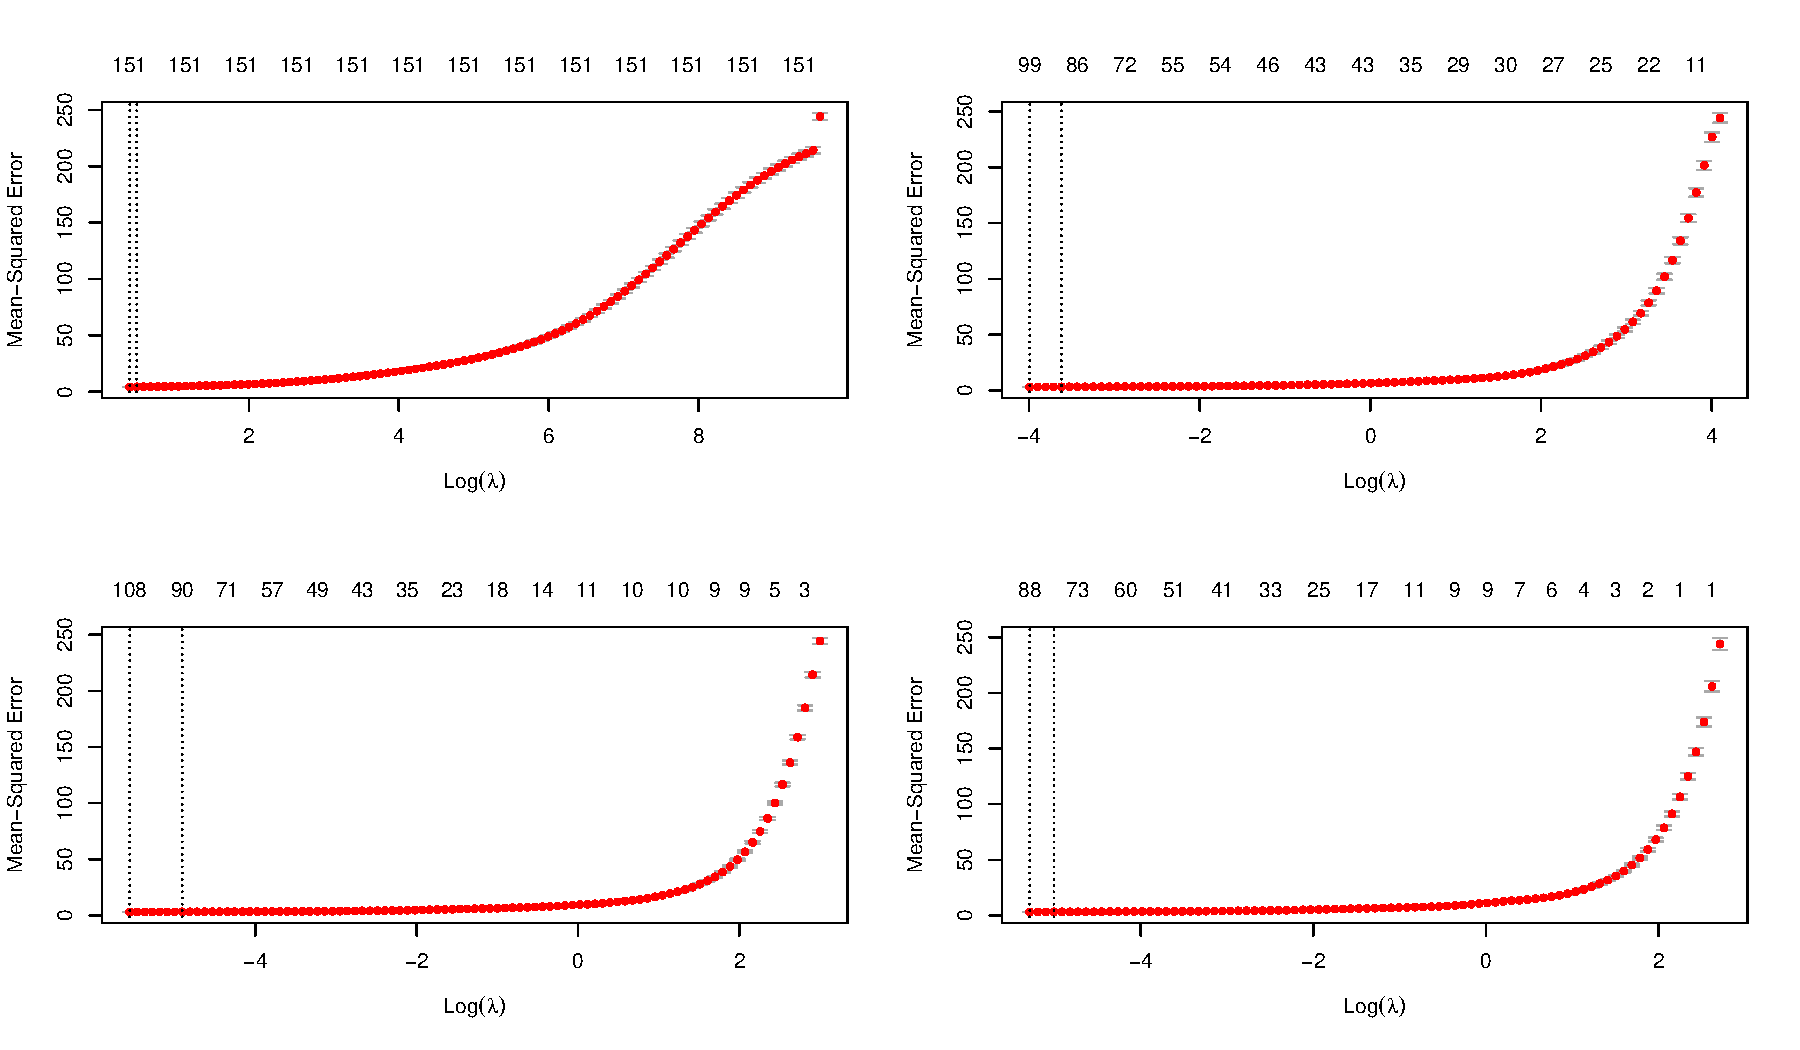
\includegraphics{TJRJCP_DuXingx_202105_files/figure-latex/unnamed-chunk-12-1} 

}

\caption{不同参数的交叉验证收敛图}\label{fig:unnamed-chunk-12}
\end{figure}

  此外,从理论上分析可以知道,岭回归约束不能对变量进行降维;而Lasso约束作为一种广泛使用的降维处理手段,在变量选择上有明显的优势且实际效果也较好。故本文采用Lasso约束进行变量降维处理。得到的变量选择结果共选取了73个变量,详见附录2。

\hypertarget{olsux56deux5f52}{%
\subsection{OLS回归}\label{olsux56deux5f52}}

\hypertarget{ux5efaux7acbolsux6a21ux578b}{%
\subsubsection{建立OLS模型}\label{ux5efaux7acbolsux6a21ux578b}}

  在描述统计的基础上,进一步分析因变量Y和各个输入自变量之间的关系。更进一步地,希望知道解释变量是怎样影响管道温度的,其影响强度如何。因此建立一个普通最小二乘回归模型对训练集数据进行拟合。

  模型的相关参数以及检验结果如下表3所示。模型整体的F-检验高度限制(P-值\textless0.001),这说明至少有一个输入变量更管道温度显著相关。模型的调整后判决系数\(R^2_{adj}=0.99\),说明输入变量对管道温度的拟合情况较优,但可能存在着较为严重的共线性问题,但本文主要考虑的是对管道温度的预测效果,故不考虑共线性问题。

\begin{longtable}[]{@{}rrrrrrrr@{}}
\caption{整体OLS模型检验结果表}\tabularnewline
\toprule
r.squared & adj.r.squared & sigma & statistic & p.value & AIC & BIC &
df.residual\tabularnewline
\midrule
\endfirsthead
\toprule
r.squared & adj.r.squared & sigma & statistic & p.value & AIC & BIC &
df.residual\tabularnewline
\midrule
\endhead
0.99 & 0.99 & 1.69 & 3951.71 & 0 & 13634.89 & 14109.06 &
3415\tabularnewline
\bottomrule
\end{longtable}

  分析每一个输入变量的t-检验结果,见表4。结果显示,X11、X12、X14、X15、X22、X29、X55、X57、X61、X65、X68、X71、X72、X85、X90、X91、X93、X95、X106、X107、X108、X121、X123、X143、X144、X145、X152变量高度不显著(检验水平\(\alpha=0.05\))。另外从表中可以发现,在高度显著的变量中,X7、X16、X111、X127在控制其他变量不变的前提下,与管道温度的变化呈现明显正相关;X18、X137在控制其他变量不变的前提下,与管道温度的变化呈现明显负相关。

\begin{longtable}[]{@{}lrrrrrr@{}}
\caption{OLS回归模型系数检验结果表}\tabularnewline
\toprule
term & estimate & std.error & statistic & p.value & conf.low &
conf.high\tabularnewline
\midrule
\endfirsthead
\toprule
term & estimate & std.error & statistic & p.value & conf.low &
conf.high\tabularnewline
\midrule
\endhead
(Intercept) & 391.16053 & 0.19598 & 1995.93770 & 0.00000 & 390.77628 &
391.54477\tabularnewline
X4 & -0.58085 & 0.19453 & -2.98590 & 0.00285 & -0.96226 &
-0.19944\tabularnewline
X7 & 1.75790 & 0.16293 & 10.78933 & 0.00000 & 1.43845 &
2.07735\tabularnewline
X8 & 0.36759 & 0.07837 & 4.69062 & 0.00000 & 0.21394 &
0.52124\tabularnewline
X10 & 0.50802 & 0.22936 & 2.21496 & 0.02683 & 0.05833 &
0.95772\tabularnewline
X11 & 0.00166 & 0.02733 & 0.06068 & 0.95161 & -0.05193 &
0.05524\tabularnewline
X12 & 2.80067 & 9.40251 & 0.29786 & 0.76583 & -15.63444 &
21.23578\tabularnewline
X14 & -6.93224 & 10.83319 & -0.63991 & 0.52228 & -28.17243 &
14.30795\tabularnewline
X15 & 2.61742 & 12.96499 & 0.20188 & 0.84002 & -22.80251 &
28.03735\tabularnewline
X16 & 6.93181 & 0.53857 & 12.87086 & 0.00000 & 5.87586 &
7.98775\tabularnewline
X18 & -7.08234 & 0.54415 & -13.01547 & 0.00000 & -8.14922 &
-6.01545\tabularnewline
X22 & -0.10814 & 0.07132 & -1.51638 & 0.12952 & -0.24797 &
0.03168\tabularnewline
X29 & 0.04709 & 0.35257 & 0.13357 & 0.89375 & -0.64417 &
0.73835\tabularnewline
X30 & 0.98567 & 0.28863 & 3.41503 & 0.00065 & 0.41977 &
1.55156\tabularnewline
X31 & -0.40061 & 0.19384 & -2.06672 & 0.03884 & -0.78067 &
-0.02056\tabularnewline
X36 & 0.82736 & 0.34483 & 2.39934 & 0.01648 & 0.15127 &
1.50345\tabularnewline
X37 & -2.40477 & 0.50781 & -4.73556 & 0.00000 & -3.40041 &
-1.40912\tabularnewline
X38 & 0.52979 & 0.30068 & 1.76201 & 0.07816 & -0.05973 &
1.11932\tabularnewline
X45 & 3.25209 & 0.34451 & 9.43968 & 0.00000 & 2.57661 &
3.92756\tabularnewline
X47 & -0.65172 & 0.21705 & -3.00260 & 0.00270 & -1.07728 &
-0.22615\tabularnewline
X55 & 0.25931 & 0.28442 & 0.91171 & 0.36199 & -0.29834 &
0.81696\tabularnewline
X57 & -0.64031 & 0.39744 & -1.61106 & 0.10726 & -1.41956 &
0.13895\tabularnewline
X61 & -0.19304 & 0.45439 & -0.42483 & 0.67098 & -1.08395 &
0.69787\tabularnewline
X65 & -0.00036 & 0.23280 & -0.00156 & 0.99876 & -0.45681 &
0.45608\tabularnewline
X66 & -2.39520 & 0.54784 & -4.37206 & 0.00001 & -3.46934 &
-1.32107\tabularnewline
X68 & -0.05471 & 0.04640 & -1.17892 & 0.23851 & -0.14569 &
0.03628\tabularnewline
X71 & 0.21570 & 0.46522 & 0.46365 & 0.64293 & -0.69644 &
1.12784\tabularnewline
X72 & 0.35011 & 0.37436 & 0.93522 & 0.34974 & -0.38388 &
1.08410\tabularnewline
X75 & 3.51418 & 0.35703 & 9.84287 & 0.00000 & 2.81417 &
4.21419\tabularnewline
X81 & 0.37467 & 0.17687 & 2.11833 & 0.03422 & 0.02789 &
0.72145\tabularnewline
X85 & 0.14427 & 0.16819 & 0.85782 & 0.39105 & -0.18548 &
0.47403\tabularnewline
X89 & -1.22455 & 0.07944 & -15.41458 & 0.00000 & -1.38031 &
-1.06880\tabularnewline
X90 & 0.50565 & 0.86963 & 0.58146 & 0.56097 & -1.19940 &
2.21070\tabularnewline
X91 & 0.84968 & 0.87053 & 0.97604 & 0.32911 & -0.85714 &
2.55650\tabularnewline
X92 & -0.38175 & 0.10824 & -3.52700 & 0.00043 & -0.59397 &
-0.16954\tabularnewline
X93 & -0.27785 & 0.25999 & -1.06869 & 0.28528 & -0.78761 &
0.23190\tabularnewline
X94 & -0.54354 & 0.29051 & -1.87096 & 0.06144 & -1.11313 &
0.02606\tabularnewline
X95 & -0.13651 & 0.10581 & -1.29008 & 0.19711 & -0.34397 &
0.07096\tabularnewline
X96 & -1.01214 & 0.19627 & -5.15694 & 0.00000 & -1.39695 &
-0.62732\tabularnewline
X101 & -0.63543 & 0.16586 & -3.83111 & 0.00013 & -0.96062 &
-0.31023\tabularnewline
X102 & -1.12815 & 0.12392 & -9.10385 & 0.00000 & -1.37112 &
-0.88519\tabularnewline
X104 & -1.39516 & 0.09751 & -14.30737 & 0.00000 & -1.58635 &
-1.20397\tabularnewline
X105 & -4.37411 & 0.30236 & -14.46656 & 0.00000 & -4.96694 &
-3.78129\tabularnewline
X106 & 0.21119 & 0.17740 & 1.19047 & 0.23395 & -0.13663 &
0.55901\tabularnewline
X107 & 0.01121 & 0.03456 & 0.32438 & 0.74567 & -0.05654 &
0.07896\tabularnewline
X108 & -0.13309 & 0.09544 & -1.39441 & 0.16329 & -0.32022 &
0.05404\tabularnewline
X109 & 0.43956 & 0.04425 & 9.93409 & 0.00000 & 0.35281 &
0.52632\tabularnewline
X110 & -0.12735 & 0.06573 & -1.93758 & 0.05276 & -0.25622 &
0.00152\tabularnewline
X111 & 8.23820 & 0.45344 & 18.16809 & 0.00000 & 7.34915 &
9.12724\tabularnewline
X112 & -0.46320 & 0.12506 & -3.70386 & 0.00022 & -0.70839 &
-0.21800\tabularnewline
X115 & 0.98531 & 0.08438 & 11.67738 & 0.00000 & 0.81987 &
1.15074\tabularnewline
X116 & 1.09287 & 0.09301 & 11.75032 & 0.00000 & 0.91051 &
1.27522\tabularnewline
X117 & 0.83392 & 0.14850 & 5.61576 & 0.00000 & 0.54277 &
1.12507\tabularnewline
X118 & 0.88522 & 0.50552 & 1.75110 & 0.08002 & -0.10593 &
1.87637\tabularnewline
X119 & -1.65403 & 0.09829 & -16.82730 & 0.00000 & -1.84675 &
-1.46131\tabularnewline
X121 & 0.04823 & 0.04018 & 1.20048 & 0.23004 & -0.03054 &
0.12700\tabularnewline
X122 & 0.77757 & 0.28551 & 2.72340 & 0.00649 & 0.21777 &
1.33737\tabularnewline
X123 & -0.03132 & 0.07326 & -0.42754 & 0.66901 & -0.17495 &
0.11231\tabularnewline
X127 & 3.49183 & 0.15759 & 22.15758 & 0.00000 & 3.18285 &
3.80081\tabularnewline
X129 & -0.15822 & 0.08482 & -1.86531 & 0.06222 & -0.32454 &
0.00809\tabularnewline
X132 & 0.43859 & 0.08750 & 5.01233 & 0.00000 & 0.26703 &
0.61015\tabularnewline
X134 & -0.35194 & 0.06463 & -5.44513 & 0.00000 & -0.47866 &
-0.22521\tabularnewline
X135 & -0.38572 & 0.07080 & -5.44786 & 0.00000 & -0.52453 &
-0.24690\tabularnewline
X137 & -2.62774 & 0.22375 & -11.74424 & 0.00000 & -3.06643 &
-2.18905\tabularnewline
X138 & -0.34832 & 0.09054 & -3.84720 & 0.00012 & -0.52584 &
-0.17081\tabularnewline
X139 & -0.36068 & 0.11187 & -3.22414 & 0.00128 & -0.58002 &
-0.14134\tabularnewline
X142 & 0.55736 & 0.14734 & 3.78273 & 0.00016 & 0.26847 &
0.84626\tabularnewline
X143 & -0.04527 & 0.09195 & -0.49232 & 0.62252 & -0.22554 &
0.13501\tabularnewline
X144 & -0.07509 & 0.07079 & -1.06084 & 0.28884 & -0.21388 &
0.06370\tabularnewline
X145 & -0.08634 & 0.06805 & -1.26881 & 0.20460 & -0.21976 &
0.04708\tabularnewline
X146 & -0.25052 & 0.11329 & -2.21128 & 0.02708 & -0.47264 &
-0.02839\tabularnewline
X147 & -1.12808 & 0.14867 & -7.58774 & 0.00000 & -1.41957 &
-0.83658\tabularnewline
X148 & 0.87794 & 0.14666 & 5.98616 & 0.00000 & 0.59039 &
1.16549\tabularnewline
X149 & 0.29724 & 0.05860 & 5.07237 & 0.00000 & 0.18235 &
0.41214\tabularnewline
X151 & -0.11161 & 0.05594 & -1.99500 & 0.04612 & -0.22129 &
-0.00192\tabularnewline
X152 & 0.01013 & 0.03026 & 0.33488 & 0.73774 & -0.04919 &
0.06946\tabularnewline
\bottomrule
\end{longtable}

\hypertarget{olsux6a21ux578bux6b8bux5deeux68c0ux9a8c}{%
\subsubsection{OLS模型残差检验}\label{olsux6a21ux578bux6b8bux5deeux68c0ux9a8c}}

\hypertarget{ux6b8bux5deeux56fe}{%
\paragraph{残差图}\label{ux6b8bux5deeux56fe}}

对于OLS模型中的随机误差向量\(\epsilon\),若高斯-马尔科夫的某些假设不成立,\(\epsilon\)的分布就会发生变化,从而导致残差e的分布变化。因此有必要对所建立模型进行残差分析,残差分析的主要思想就是通过对e的表现加以研究,包括零均值、同方差、独立性,此处关于高斯-马尔科夫假设不进行详细阐述。从预测角度定义残差:

\[\sigma_i=Y_i-x_i'\hat{\beta}(i), i=1,...,n\]

  由于量纲和度量单位的影响,直接进行比较普通残差是不适宜的,为此将他们标准化。有两种重要的标准化残差定义方式就是内学生化残差和外学生化残差。本文同时给出了这两种残差的残差图,见图6。

  由残差图可以发现,这些残差大致都落在(-2,2)的水平带域内,且不存在任何的趋势。这时数据与假设\(N(0,1)\)没有不一致的征兆,可以认为这个假设基本上是合理的。

\begin{figure}

{\centering 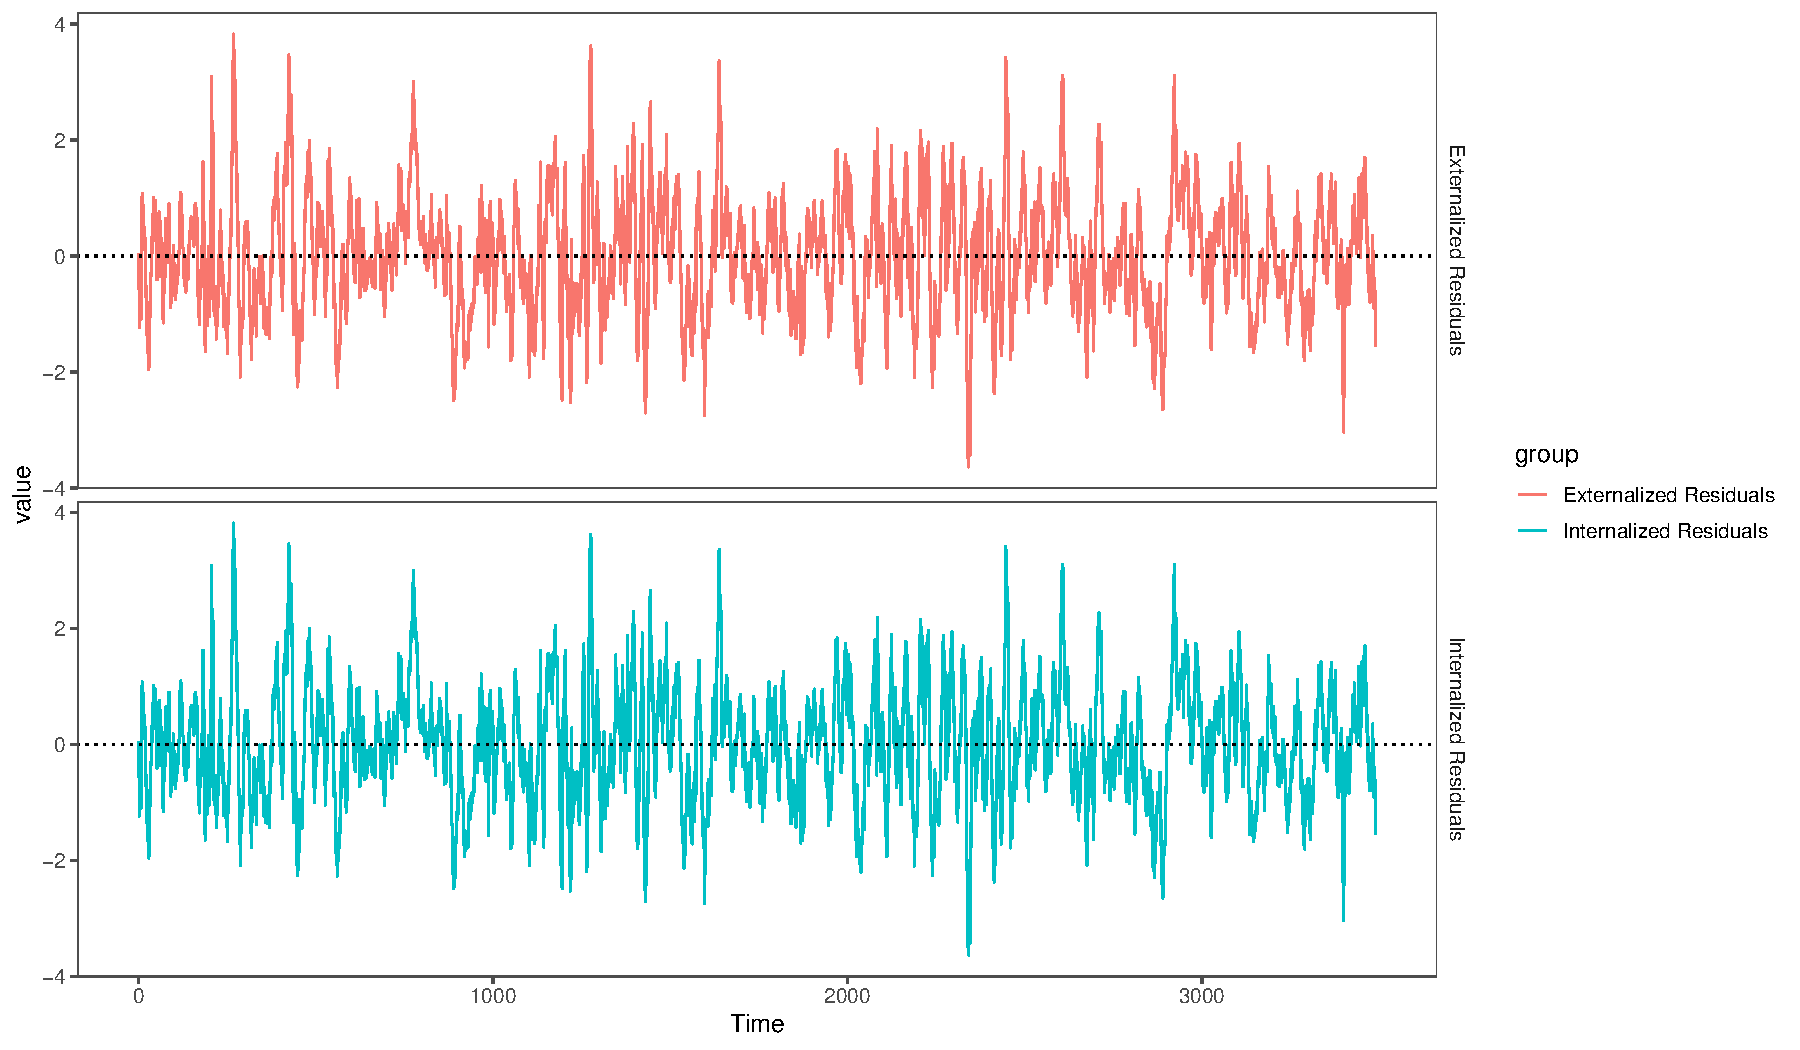
\includegraphics{TJRJCP_DuXingx_202105_files/figure-latex/unnamed-chunk-17-1} 

}

\caption{拟合模型的标准化学生残差图}\label{fig:unnamed-chunk-17}
\end{figure}

\hypertarget{ux6b63ux6001ux6027ux68c0ux9a8c}{%
\paragraph{正态性检验}\label{ux6b63ux6001ux6027ux68c0ux9a8c}}

图示法虽然能够较为直接的进行残差分析,但具有一定的主观性。因此,需要进一步通过假设检验的方式对残差进行正态性检验,见表5。本文采用R语言的shapiro.text函数进行正态性检验,检验显著性P-值远小于0.001,故拒绝原假设,接受残差不服从正态分布的假设。

\begin{longtable}[]{@{}rrl@{}}
\caption{残差的正态性检验结果表}\tabularnewline
\toprule
statistic & p.value & method\tabularnewline
\midrule
\endfirsthead
\toprule
statistic & p.value & method\tabularnewline
\midrule
\endhead
0.9964769 & 3e-07 & Shapiro-Wilk normality test\tabularnewline
\bottomrule
\end{longtable}

\hypertarget{olsux6a21ux578bux62dfux5408}{%
\subsubsection{OLS模型拟合}\label{olsux6a21ux578bux62dfux5408}}

  用此模型对采样数据进行拟合并在测试集上进行预测,黑色的线代表实际的平均管道温度,绿色的线代表对建模所用数据进行回代拟合,红色的线代表对测试集的采样数据进行外样本预测,见图7。

\begin{figure}

{\centering 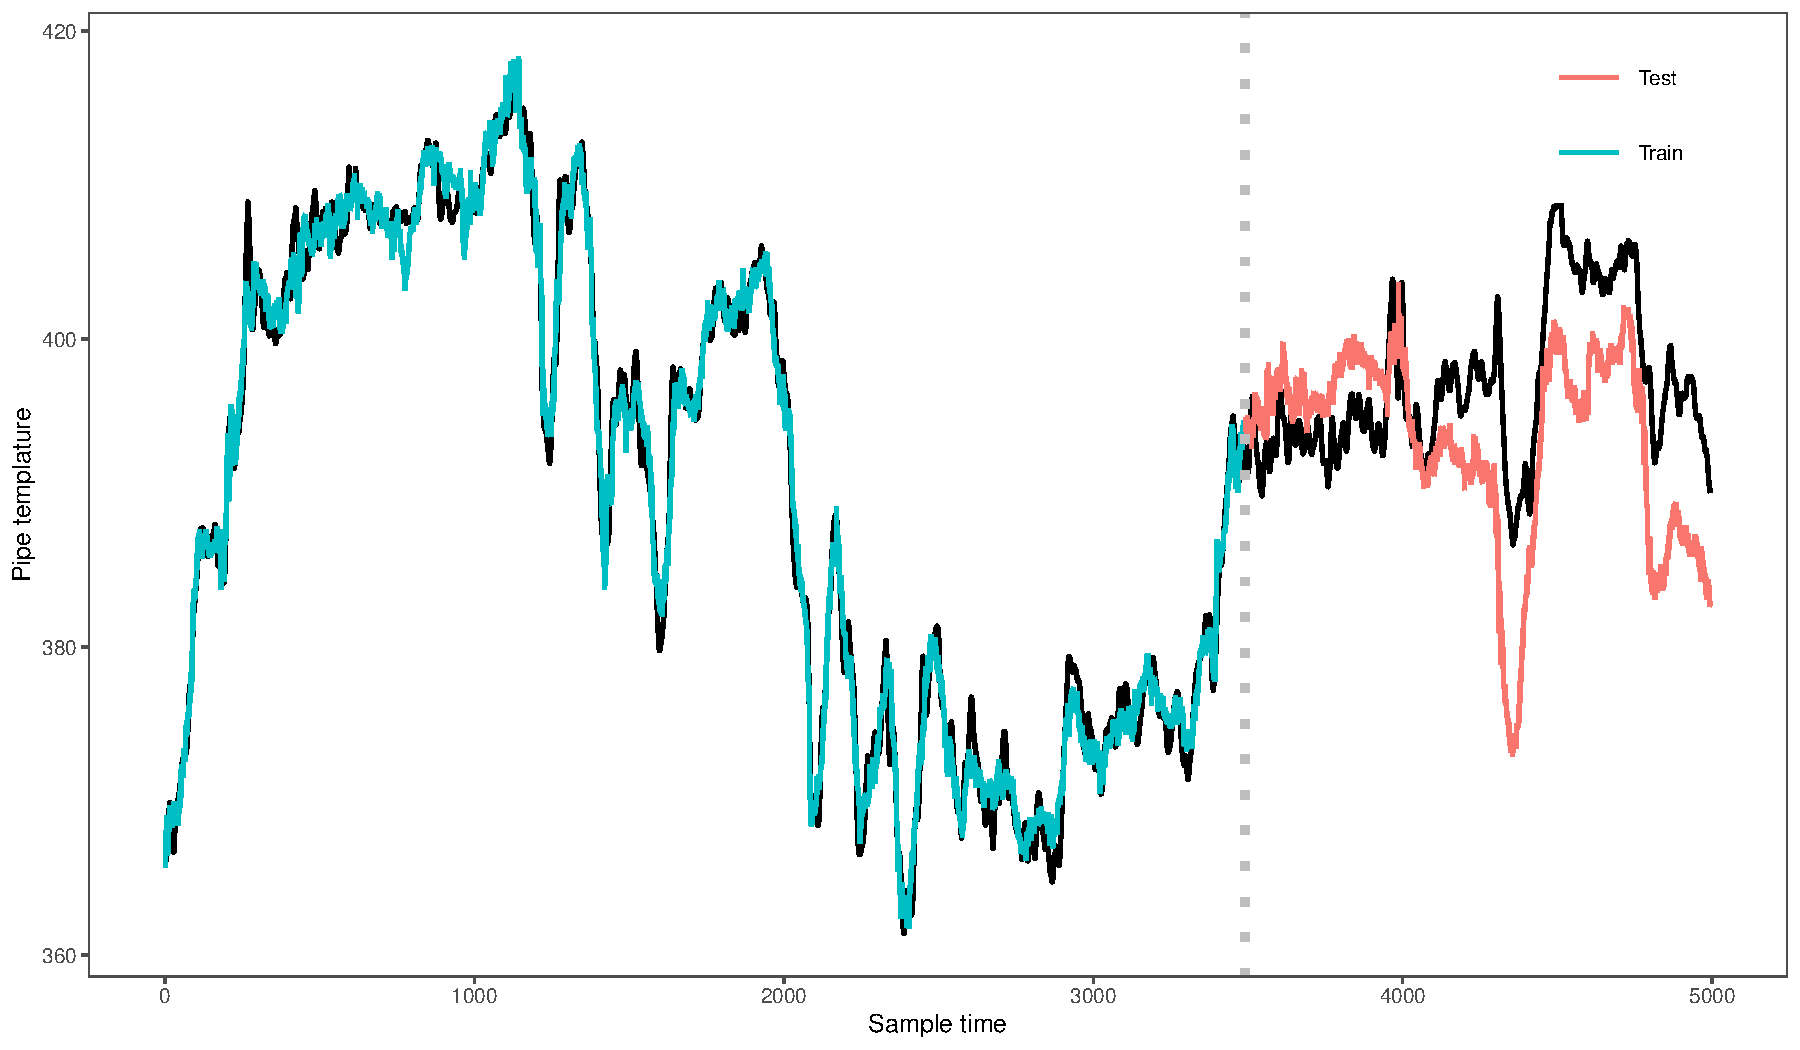
\includegraphics{TJRJCP_DuXingx_202105_files/figure-latex/unnamed-chunk-19-1} 

}

\caption{OLS模型拟合效果图}\label{fig:unnamed-chunk-19}
\end{figure}

  从图形上来看,在训练集数据上预测效果拟合较好,但是在测试集数据上的预测效果明显差一些,但是对与管道温度的整体走势波动也能进行预测。并且对波峰波谷等转折点也能较好的预测。

  此外通过计算拟合和预测效果的一些评估指标如下表所示。当然为了衡量预测与实际数据之间的差距程度有各种各样的专业指标来评估,例如平均绝对误差,均方误差,决定系数,误差平方和,交叉熵误差等。本文采用了均方误差、误差平方和、平均绝对误差三个指标来衡量。

  均方误差(MSE):

\[MSE=\frac{\sum_{i=1}^m(f(x)-y_i)^2}{m}\]

  平均绝对误差(MAE):

\[MAE=\frac{\sum_{i=1}^m|f(x)-y_i|}{m}\]

  误差平方和(SSE):

\[SSE=\sum_{i=1}^m(f(x)-y_i)^2\]

 计算结果见表6。训练集的残差平方和为10239.28,均方误差为2.93,绝对值残差和为4708.62;测试集的残差平方和为60747.91,均方误差为40.42,绝对值残差和为8045。68。可以发现,训练集上的均方误差远远小于测试集上的,当然均方误差由于经过平方之后拉大了实际上的差距。从绝对值误差平方和可以看出测试集上的误差接近与训练集的两倍。但是由于整体样本量较多,实际上对于单个样本的管道温度误差较小,结果可以接受。

\begin{longtable}[]{@{}lrrr@{}}
\caption{OLS回归模型评估结果}\tabularnewline
\toprule
Data & MSE & SSE & SAE\tabularnewline
\midrule
\endfirsthead
\toprule
Data & MSE & SSE & SAE\tabularnewline
\midrule
\endhead
Train Data & 2.783577 & 9717.468 & 4586.289\tabularnewline
Test Data & 45.926135 & 69026.981 & 8599.783\tabularnewline
\bottomrule
\end{longtable}

\hypertarget{ridgeux56deux5f52}{%
\subsection{Ridge回归}\label{ridgeux56deux5f52}}

\hypertarget{ux5efaux7acbux6a21ux578b}{%
\subsubsection{建立模型}\label{ux5efaux7acbux6a21ux578b}}

  岭回归估计(Ridge)是一种专用于共线性数据分析的有偏估计回归方法,实质上是一种改良的最小二乘估计法
。通过放弃最小二乘的无偏性,以损失部分信息、降低精度为代价获得回归系数更为符合实际的回归方法,对病态数据的耐受性远远高于最小二乘法。

  思想是在原先的\(\beta\)的最小二乘估计中加入一个小扰动\(\lambda\),使原先无法求广义逆的情况变成可以求出其广义逆,使得问题稳定并得以求解。

\[\hat{\beta}_{ridge}=arg min_{\beta}\left(\sum_{i=1}^N(y_i-\beta_0-\sum_{j=1}^px_{ij}\beta_j)^2+\lambda\sum_{j=1}^p\beta_j^2\right)\]

  上式就是称为关于岭回归\(\lambda\)的岭回归估计。后面这一项\(\lambda\sum_{j=1}^p\beta_j^2\)称为惩罚函数,它保证了\(\beta\)值不会变的很大。岭参数\(\lambda\)不同,岭回归系数也会不同。因此,我们对训练集数据建立岭回归模型,首先回归不同的\(\lambda\)下不同的岭回归系数,得到岭迹图见图8。

\begin{figure}

{\centering 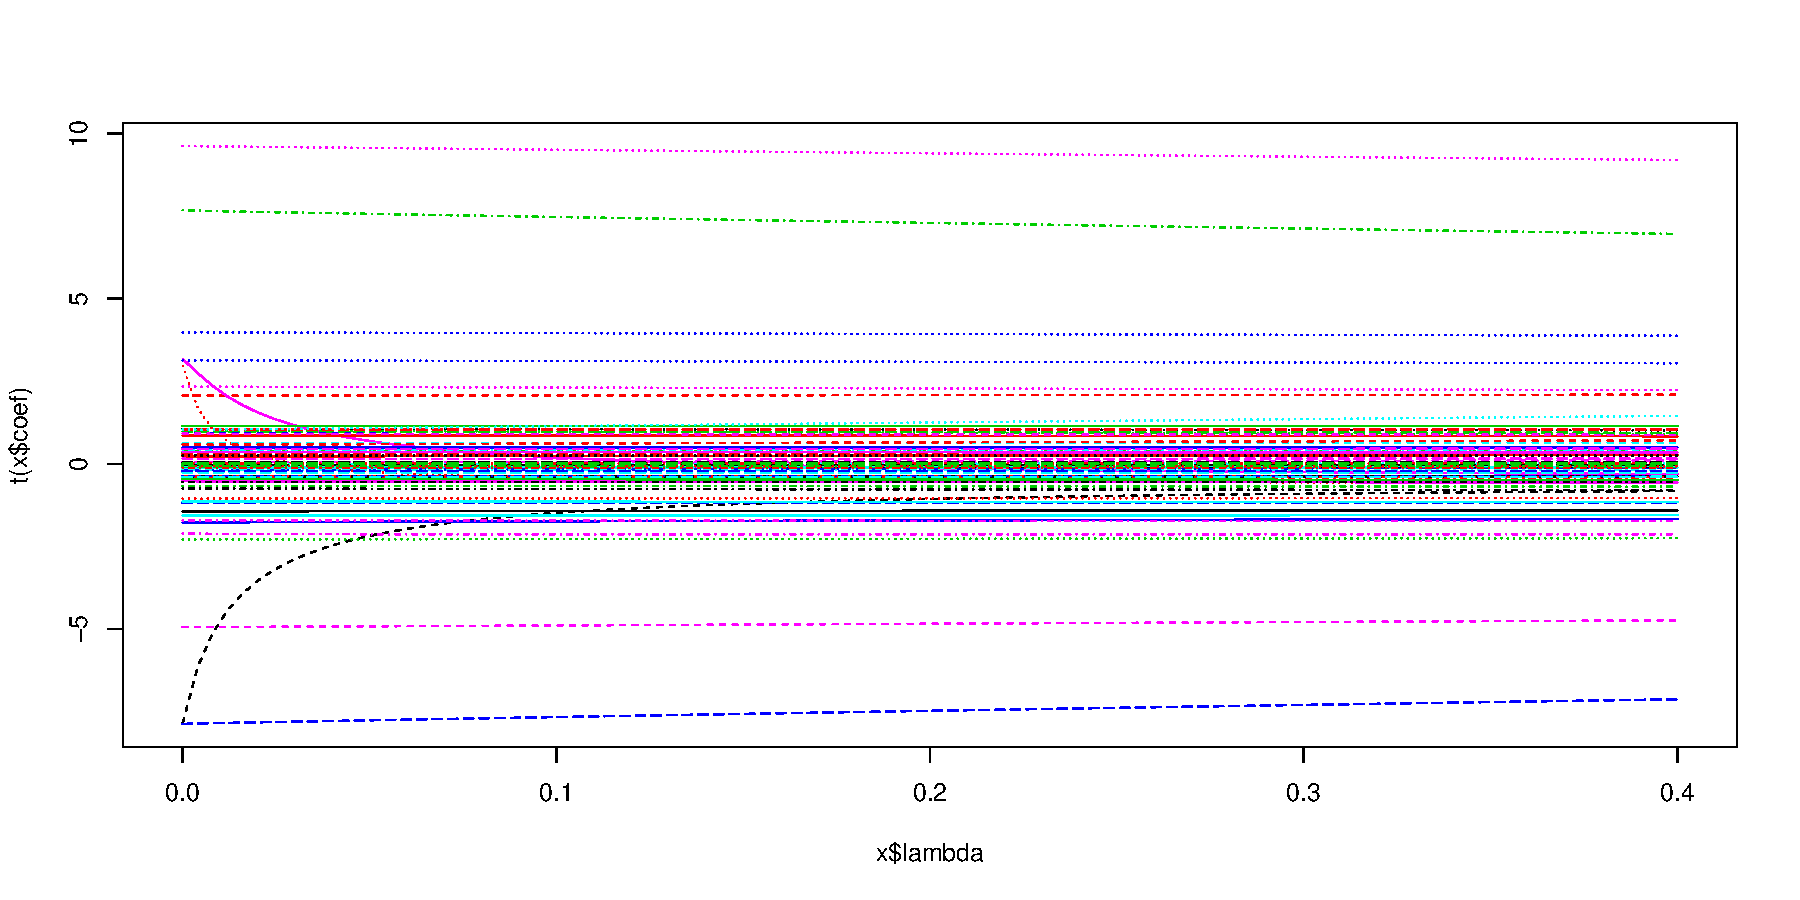
\includegraphics{TJRJCP_DuXingx_202105_files/figure-latex/unnamed-chunk-21-1} 

}

\caption{Ridge回归模型岭迹图}\label{fig:unnamed-chunk-21}
\end{figure}

  从图中可见,在\(\lambda\)很小时,通常各\(\beta\)系数取值较大;而如果\(\lambda=0\),则
根普通意义的多元线性回归的最小二乘解完全一样;当\(\lambda\)略有增大,则各\(\beta\)系数取值迅速减小,即从不稳定趋于稳定。上图中的变化实际上并没有其他相关文献中的那么呈现喇叭状的岭迹图,说明原始的最小二乘解中的多重共线性不严重,或者几乎不存在多重共线性。但是我们主要考虑的是用岭回归方法进行建模预测,所以此处不影响后续考虑分析。

  一个合适较好的\(\lambda\)需要满足以下条件:各回归系数的岭估计基本稳定;用最小二乘估计时符号不合理的回归系数其岭估计的符号变得合理;回归系数没有不合乎实际意义的值;残差平方和增大不太多,一般\(\lambda\)越大,系数\(\beta\)会出现稳定的假象,但是残差平方和也会更大。对于最佳参数的选择有不同方法,但是结果差异较大,这是岭回归的弱点之一。R中也提供了几种选择准则:kHKB、kLW、lambdaGCV。本文按照kHKB的准则选取\(\lambda=0.5290778\)。并在此\(\lambda\)的基础上建立模型。得到系数估计见表7。

\begin{longtable}[]{@{}rrlrr@{}}
\caption{Ridge回归模型系数检验结果表}\tabularnewline
\toprule
lambda & GCV & term & estimate & scale\tabularnewline
\midrule
\endfirsthead
\toprule
lambda & GCV & term & estimate & scale\tabularnewline
\midrule
\endhead
0.5290788 & 0.0008323 & X4 & -0.5024149 & 0.8935214\tabularnewline
0.5290788 & 0.0008323 & X7 & 2.1013410 & 1.1776347\tabularnewline
0.5290788 & 0.0008323 & X8 & 0.3691742 & 0.9603131\tabularnewline
0.5290788 & 0.0008323 & X10 & 0.5057741 & 0.9629931\tabularnewline
0.5290788 & 0.0008323 & X11 & 0.0017280 & 1.0853259\tabularnewline
0.5290788 & 0.0008323 & X12 & -0.3571988 & 1.1328747\tabularnewline
0.5290788 & 0.0008323 & X14 & -0.7603741 & 1.1324429\tabularnewline
0.5290788 & 0.0008323 & X15 & -0.5817843 & 1.1322578\tabularnewline
0.5290788 & 0.0008323 & X16 & 6.7647440 & 1.1080880\tabularnewline
0.5290788 & 0.0008323 & X18 & -6.9237323 & 1.1121611\tabularnewline
0.5290788 & 0.0008323 & X22 & -0.1173548 & 1.1962978\tabularnewline
0.5290788 & 0.0008323 & X29 & 0.1164576 & 1.0721913\tabularnewline
0.5290788 & 0.0008323 & X30 & 1.0006100 & 1.0686677\tabularnewline
0.5290788 & 0.0008323 & X31 & -0.4709983 & 1.1223700\tabularnewline
0.5290788 & 0.0008323 & X36 & 0.9249425 & 1.1710010\tabularnewline
0.5290788 & 0.0008323 & X37 & -1.6375337 & 0.7405153\tabularnewline
0.5290788 & 0.0008323 & X38 & 0.6419679 & 1.1725393\tabularnewline
0.5290788 & 0.0008323 & X45 & 2.2002650 & 0.7188259\tabularnewline
0.5290788 & 0.0008323 & X47 & -0.8112250 & 1.1385512\tabularnewline
0.5290788 & 0.0008323 & X55 & 0.2791919 & 1.1510370\tabularnewline
0.5290788 & 0.0008323 & X57 & -0.4983707 & 0.7153791\tabularnewline
0.5290788 & 0.0008323 & X61 & -0.0981981 & 1.0191294\tabularnewline
0.5290788 & 0.0008323 & X65 & 0.0075782 & 0.8972643\tabularnewline
0.5290788 & 0.0008323 & X66 & -2.1296949 & 0.8805054\tabularnewline
0.5290788 & 0.0008323 & X68 & -0.0538015 & 0.9919866\tabularnewline
0.5290788 & 0.0008323 & X71 & 0.2774608 & 1.0317235\tabularnewline
0.5290788 & 0.0008323 & X72 & 0.3685630 & 1.0418374\tabularnewline
0.5290788 & 0.0008323 & X75 & 3.8493576 & 1.1333168\tabularnewline
0.5290788 & 0.0008323 & X81 & 0.4372453 & 1.1315021\tabularnewline
0.5290788 & 0.0008323 & X85 & 0.1575223 & 1.0586309\tabularnewline
0.5290788 & 0.0008323 & X89 & -1.3965477 & 1.1770960\tabularnewline
0.5290788 & 0.0008323 & X90 & 0.7396067 & 1.1551456\tabularnewline
0.5290788 & 0.0008323 & X91 & 0.8552335 & 1.1591196\tabularnewline
0.5290788 & 0.0008323 & X92 & -0.3819846 & 1.0324867\tabularnewline
0.5290788 & 0.0008323 & X93 & -0.2626921 & 0.9238216\tabularnewline
0.5290788 & 0.0008323 & X94 & -0.5701121 & 0.9656632\tabularnewline
0.5290788 & 0.0008323 & X95 & -0.0860935 & 0.4855904\tabularnewline
0.5290788 & 0.0008323 & X96 & -1.0389821 & 1.0449909\tabularnewline
0.5290788 & 0.0008323 & X101 & -0.6991791 & 1.0555196\tabularnewline
0.5290788 & 0.0008323 & X102 & -1.1616452 & 1.0522967\tabularnewline
0.5290788 & 0.0008323 & X104 & -1.5460359 & 1.1267009\tabularnewline
0.5290788 & 0.0008323 & X105 & -4.6774222 & 1.1304400\tabularnewline
0.5290788 & 0.0008323 & X106 & 0.2424159 & 1.1812707\tabularnewline
0.5290788 & 0.0008323 & X107 & 0.0101997 & 0.9272312\tabularnewline
0.5290788 & 0.0008323 & X108 & -0.0718186 & 0.6282127\tabularnewline
0.5290788 & 0.0008323 & X109 & 0.4991405 & 1.1341835\tabularnewline
0.5290788 & 0.0008323 & X110 & -0.0589414 & 0.4489232\tabularnewline
0.5290788 & 0.0008323 & X111 & 9.0796562 & 1.1680036\tabularnewline
0.5290788 & 0.0008323 & X112 & -0.5511791 & 1.1825085\tabularnewline
0.5290788 & 0.0008323 & X115 & 1.0473650 & 1.0532798\tabularnewline
0.5290788 & 0.0008323 & X116 & 1.1384111 & 1.0519541\tabularnewline
0.5290788 & 0.0008323 & X117 & 0.8319923 & 1.1040520\tabularnewline
0.5290788 & 0.0008323 & X118 & 1.5706048 & 1.1669537\tabularnewline
0.5290788 & 0.0008323 & X119 & -1.7407824 & 1.0351108\tabularnewline
0.5290788 & 0.0008323 & X121 & 0.0441537 & 0.9427944\tabularnewline
0.5290788 & 0.0008323 & X122 & 0.8267476 & 1.0952375\tabularnewline
0.5290788 & 0.0008323 & X123 & -0.0383046 & 1.0970817\tabularnewline
0.5290788 & 0.0008323 & X127 & 3.0180451 & 0.8981289\tabularnewline
0.5290788 & 0.0008323 & X129 & -0.1828876 & 1.1555520\tabularnewline
0.5290788 & 0.0008323 & X132 & 0.4650212 & 1.0136909\tabularnewline
0.5290788 & 0.0008323 & X134 & -0.3900758 & 1.0875998\tabularnewline
0.5290788 & 0.0008323 & X135 & -0.4023739 & 0.9996595\tabularnewline
0.5290788 & 0.0008323 & X137 & -2.2413094 & 0.8714826\tabularnewline
0.5290788 & 0.0008323 & X138 & -0.3738689 & 1.0608146\tabularnewline
0.5290788 & 0.0008323 & X139 & -0.3892464 & 1.1141027\tabularnewline
0.5290788 & 0.0008323 & X142 & 0.3302206 & 0.6510141\tabularnewline
0.5290788 & 0.0008323 & X143 & -0.0364446 & 0.9038822\tabularnewline
0.5290788 & 0.0008323 & X144 & -0.0777554 & 0.9404008\tabularnewline
0.5290788 & 0.0008323 & X145 & -0.0697477 & 0.8108473\tabularnewline
0.5290788 & 0.0008323 & X146 & -0.2177336 & 0.8665161\tabularnewline
0.5290788 & 0.0008323 & X147 & -1.1650331 & 1.0175172\tabularnewline
0.5290788 & 0.0008323 & X148 & 0.8700664 & 1.0389954\tabularnewline
0.5290788 & 0.0008323 & X149 & 0.2586349 & 0.8810920\tabularnewline
0.5290788 & 0.0008323 & X151 & -0.1253845 & 1.0887538\tabularnewline
0.5290788 & 0.0008323 & X152 & 0.0055651 & 1.1706949\tabularnewline
\bottomrule
\end{longtable}

\hypertarget{ridgeux6a21ux578bux62dfux5408}{%
\subsubsection{Ridge模型拟合}\label{ridgeux6a21ux578bux62dfux5408}}

  用此模型对采样数据进行拟合并在测试集上进行预测,黑色的线代表实际的平均管道温度,绿色的线代表对建模所用数据进行回代拟合,红色的线代表对测试集的采样数据进行外样本预测,如图9所示。

\begin{figure}

{\centering 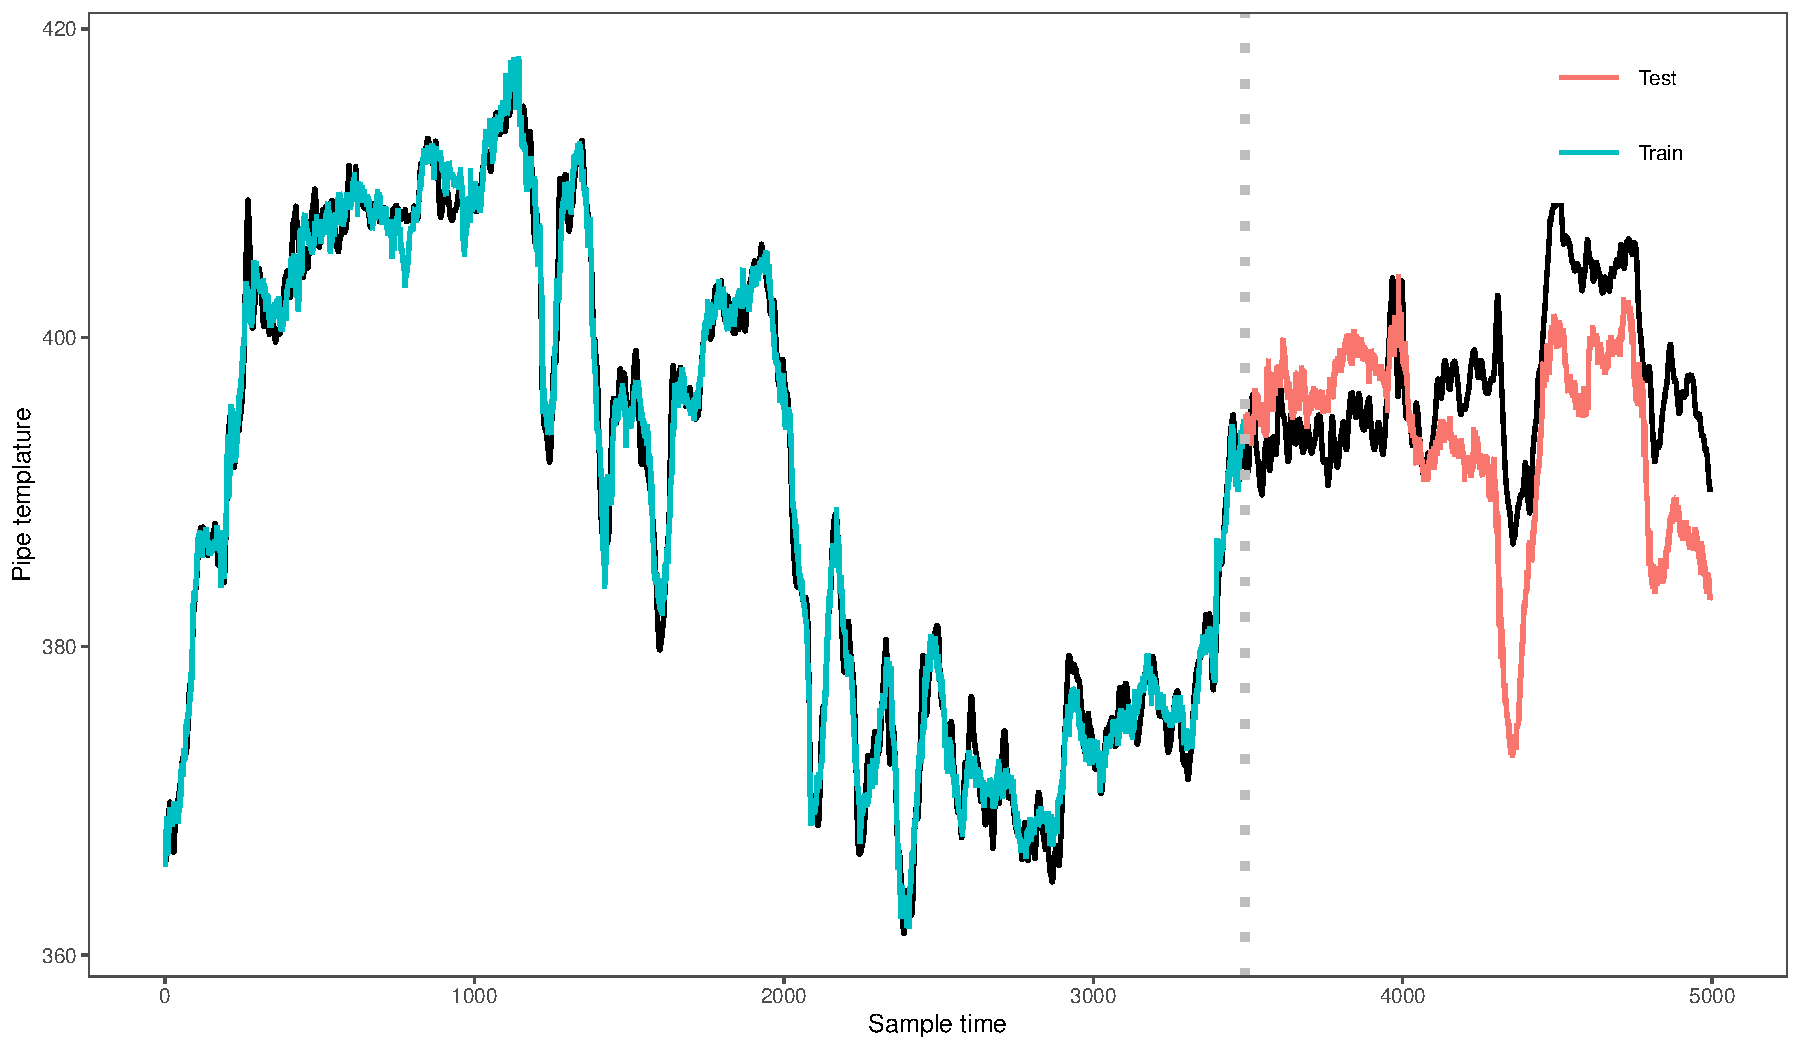
\includegraphics{TJRJCP_DuXingx_202105_files/figure-latex/unnamed-chunk-25-1} 

}

\caption{Ridge模型拟合效果图}\label{fig:unnamed-chunk-25}
\end{figure}

  从图形上来看,在训练集数据上预测效果拟合较好,但是在测试集数据上的预测效果明显差一些,但是对与管道温度的整体走势波动也能进行预测。并且对波峰波谷等转折点也能较好的预测。

  此外通过计算拟合和预测效果的一些评估指标见表8所示。从表中得到,训练集的残差平方和为9728.97,均方误差为2.79,绝对值残差和为4592.21;测试集的残差平方和为65908.22,均方误差为43.85,绝对值残差和为8400.26。可以发现,训练集上的均方误差远远小于测试集上的,当然均方误差由于经过平方之后拉大了实际上的差距。从绝对值误差平方和可以看出测试集上的误差接近与训练集的两倍。但是由于整体样本量较多,实际上对于单个样本的管道温度误差较小,结果可以接受。

\begin{longtable}[]{@{}lrrr@{}}
\caption{Ridge回归模型评估结果}\tabularnewline
\toprule
Data & MSE & SSE & SAE\tabularnewline
\midrule
\endfirsthead
\toprule
Data & MSE & SSE & SAE\tabularnewline
\midrule
\endhead
Train Data & 2.786872 & 9728.969 & 4592.207\tabularnewline
Test Data & 43.851114 & 65908.224 & 8400.256\tabularnewline
\bottomrule
\end{longtable}

\hypertarget{ux6a21ux578bux7ed3ux679c}{%
\subsection{模型结果}\label{ux6a21ux578bux7ed3ux679c}}

  从上述建立的OLS、Ridge两个回归模型效果可以看出。虽然OLS在总的残差平方和上面要小,但是Ridge回归对于变量的解释性、合理性更强。而管道温度的调控需要实际的操作变量来调整,如果操作过程对管道温度影响方向的异常,可能产生不可预料的后果。因此本文采用更符合实际的ridge回归模型。

应用到均值温度的模型表达式为:

\[Y=-0.50X_4+2.10X_7+0.37X_8+0.51X_{10}+0.001X_{11}+...+0.87X_{148}+0.25X_{149}-0.13X_{151}+0.01X_{152}\]

  对ridge回归模型得到的变量系数估计有着重要的实际意义。当系数大于0时,代表该变量对管道温度产生正的影响;当系数小于0时,代表该变量对管道温度产生负的影响。而系数的绝对值大小代表着影响的强度。因此为了更直接的观察回归模型结果的系数的实际意义,对估计的系数绘制了散点图如图10所示。

\begin{figure}

{\centering 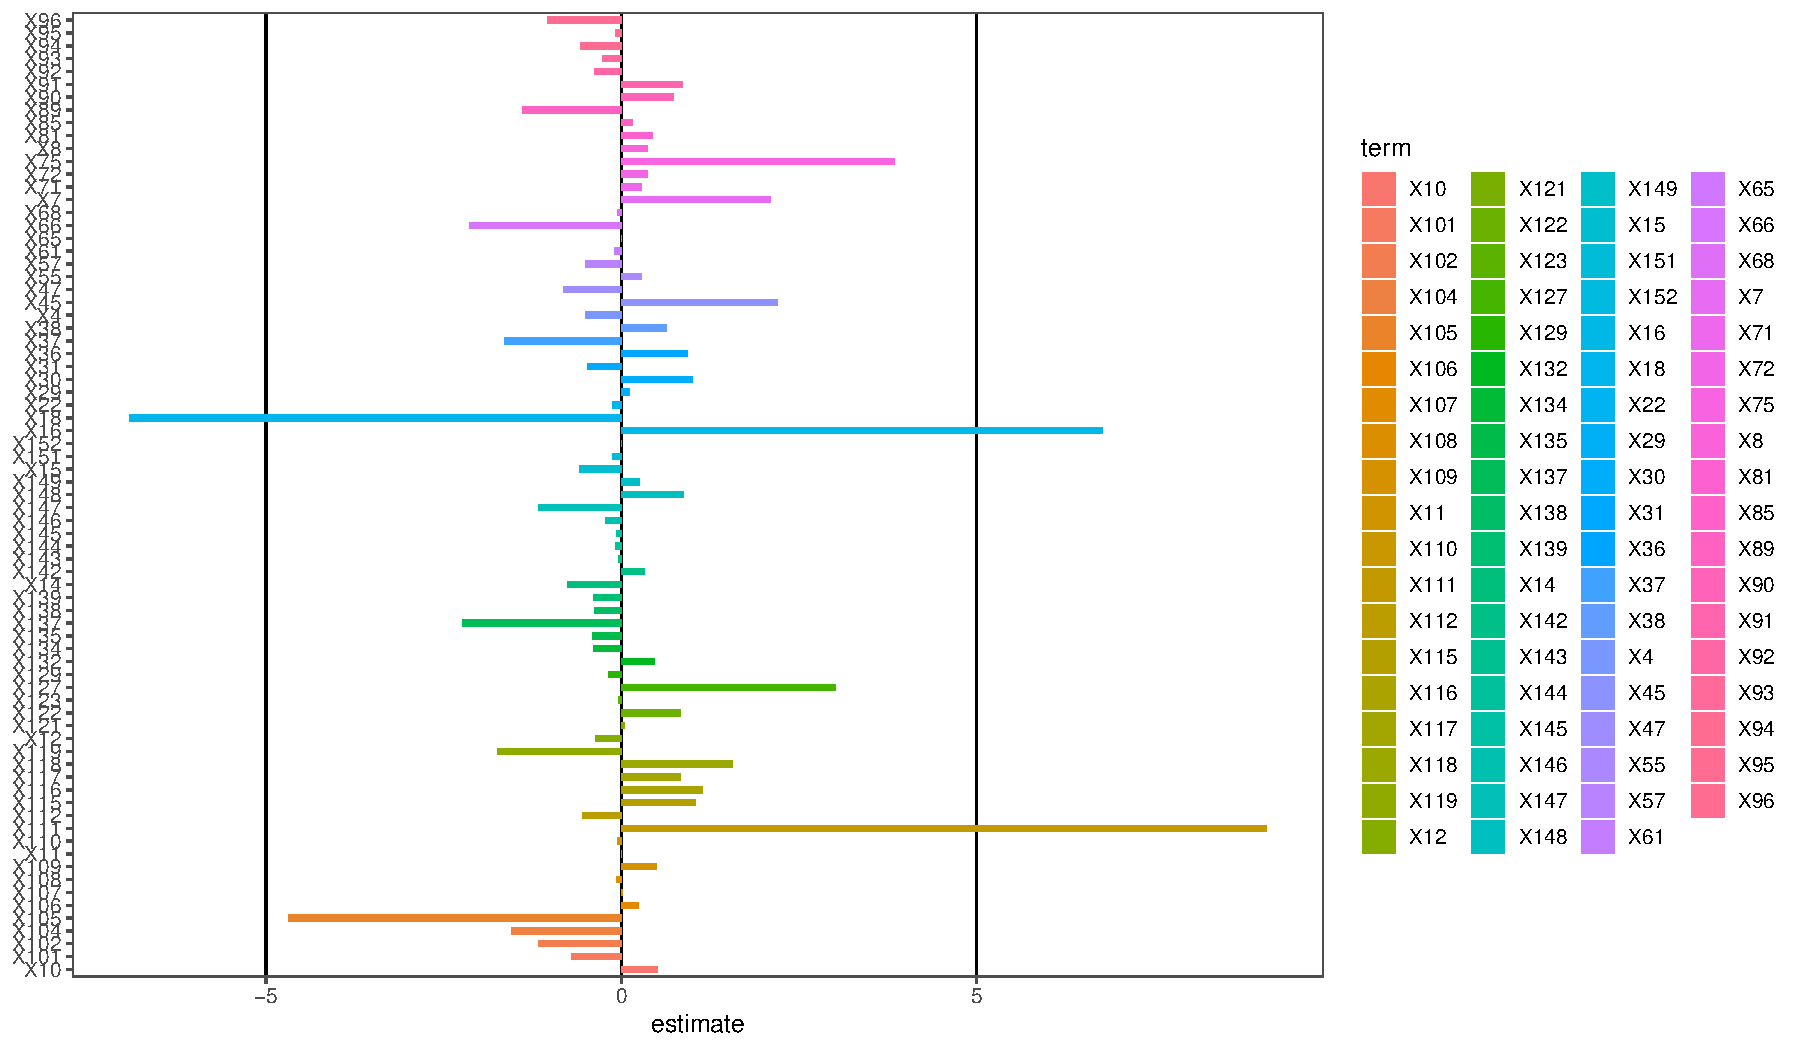
\includegraphics{TJRJCP_DuXingx_202105_files/figure-latex/unnamed-chunk-27-1} 

}

\caption{自变量系数的散点图}\label{fig:unnamed-chunk-27}
\end{figure}

  从图中可以发现,4角BC层二次风调节挡板位置反馈、1角A层二次风调节挡板位置反馈、A磨入口热一次风电调挡板位置、省煤器出口温度2、分离器出口汽温定值、A磨分离器风粉混合物温度2的系数值较大,即说明这几个变量为重要的操作变量。且管道温度与省煤器出口温度2为正相关,且该变量对管道温度影响在所有变量中影响最为强烈;A磨入口热一次风电调挡板位置对管道温度的影响呈现强烈的负相关。

\hypertarget{ux6a21ux578bux5e94ux7528}{%
\subsection{模型应用}\label{ux6a21ux578bux5e94ux7528}}

  上述的模型为管道均值温度建模,实际上我们需要对各个管道温度建立有效的模型。因此,将上述模型应用到10个管道温度数据上,得到10个管道的拟合预测效果图,见附录3。

  从应用结果可以发现,整体上对于模型应用的效果较好,且对于超温现象能够较好的识别和拟合。

\hypertarget{ux7ed3ux8bba}{%
\section{结论}\label{ux7ed3ux8bba}}

  时间序列平稳性检验可以很好地评价管道温度工作曲线的稳定性,使分析结果更具有合理性。综合比较线性回归,岭回归模型,由于岭回归在变量实际含义的解释方面有着更优秀的表现,因此采用线性回归模型进行结果,结果更加准确。

  虽然目前所得到的模型能够较好的拟合,但是由于所用模型线性模型较为简单,且未考虑时间因素的影响。所以残差存在非正态性,实际中可以考虑其他非线性模型和考虑时间序列分析。例如进行多元非线性拟合出最优方程或者建立LSTM神经网络建立水冷壁管道温度变化规律的数学模型,从而得到的优化模型更为准确。

\newpage

\hypertarget{ux53c2ux8003ux6587ux732e}{%
\section{参考文献}\label{ux53c2ux8003ux6587ux732e}}

\begin{quote}
{[}1{]}仙树祥.
大容量``W''火焰超临界锅炉优化运行技术研究{[}D{]}.华北电力大学,2015.
\end{quote}

\begin{quote}
{[}2{]}陈世杰,唐秋华.优化神经网络用电量预测性能的多元线性回归方法{[}J{]}.机械设计与制造,2019(06):17-21.
\end{quote}

\begin{quote}
{[}3{]}Neeraj Kumar, Ganesh Upadhyay and Pankaj Kumar. Comparative
Performance of Multiple Linear Regression and Artificial Neural Network
Based Models in Estimation of Evaporation {[}J{]}Advances in Research,
2017,11
\end{quote}

\begin{quote}
{[}4{]}李雷,赵柏森.基于人工神经网络和遗传算法的封头成形工艺参数多目标优化{[}J/OL{]}.锻压技术,2021(05):39-45{[}2021-05-23{]}.
\end{quote}

\begin{quote}
{[}5{]}
陈士华,马益平,方健美.遗传算法在智能配电网故障定位应用分析{[}J{]}.能源与环保,2017,39(12):219-222
\end{quote}

\newpage

\hypertarget{ux9644ux5f55}{%
\section{附录}\label{ux9644ux5f55}}

\hypertarget{ux9644ux5f55ux4e00ux81eaux53d8ux91cfux57faux672cux7edfux8ba1ux7279ux5f81ux8868}{%
\subsection{附录一:自变量基本统计特征表}\label{ux9644ux5f55ux4e00ux81eaux53d8ux91cfux57faux672cux7edfux8ba1ux7279ux5f81ux8868}}

\begin{longtable}[]{@{}lrrrrrrrrr@{}}
\toprule
Variables & Mean & Std & Max & Min & Q25 & Q50 & Q75 & PNum &
TNum\tabularnewline
\midrule
\endhead
X1 & 129.10 & 23.34 & 180.13 & 87.34 & 142.36 & 128.54 & 107.70 & 971 &
970\tabularnewline
X10 & 23.09 & 24.65 & 50.45 & 0.45 & 50.36 & 0.90 & 0.81 & 1621 &
1670\tabularnewline
X100 & 30.23 & 2.00 & 36.18 & 23.77 & 31.90 & 30.22 & 28.59 & 1260 &
1261\tabularnewline
X101 & 18.27 & 21.93 & 65.50 & -0.40 & 37.28 & 6.25 & -0.36 & 914 &
1246\tabularnewline
X102 & 546.47 & 37.80 & 746.13 & 437.94 & 567.48 & 538.61 & 522.35 &
1587 & 1584\tabularnewline
X103 & 30.19 & 2.11 & 41.58 & 23.65 & 31.49 & 29.70 & 28.98 & 1503 &
1509\tabularnewline
X104 & 9.51 & 16.25 & 53.69 & -0.26 & 15.39 & -0.20 & -0.22 & 629 &
1299\tabularnewline
X105 & 11.89 & 24.61 & 68.80 & -0.47 & -0.30 & -0.30 & -0.34 & 1026 &
661\tabularnewline
X106 & 42.03 & 32.29 & 99.66 & -0.50 & 72.90 & 43.49 & -0.40 & 1159 &
1085\tabularnewline
X107 & 99.51 & 0.59 & 99.79 & 88.26 & 99.78 & 99.76 & 99.34 & 2267 &
1372\tabularnewline
X108 & 99.13 & 0.36 & 99.75 & 94.06 & 99.28 & 98.98 & 98.84 & 1171 &
1286\tabularnewline
X109 & 99.51 & 2.42 & 100.24 & 79.55 & 100.21 & 100.20 & 100.19 & 2056 &
878\tabularnewline
X11 & 50.16 & 0.12 & 50.45 & 49.38 & 50.24 & 50.17 & 50.10 & 1663 &
1662\tabularnewline
X110 & 99.63 & 0.47 & 99.68 & 84.40 & 99.67 & 99.67 & 99.67 & 2671 &
917\tabularnewline
X111 & 274.64 & 12.04 & 296.72 & 254.31 & 281.95 & 277.29 & 265.39 & 770
& 729\tabularnewline
X112 & 226.93 & 41.38 & 310.00 & 178.07 & 245.28 & 227.23 & 182.54 &
1178 & 1965\tabularnewline
X113 & 15.75 & 2.81 & 21.52 & 11.53 & 17.47 & 15.77 & 12.87 & 792 &
785\tabularnewline
X114 & 2.24 & 0.41 & 3.14 & 1.69 & 2.39 & 2.22 & 1.89 & 1215 &
1162\tabularnewline
X115 & 563.98 & 5.83 & 570.84 & 538.27 & 568.12 & 566.42 & 561.91 & 515
& 524\tabularnewline
X116 & 550.08 & 7.58 & 563.64 & 527.19 & 555.38 & 551.31 & 546.17 & 308
& 290\tabularnewline
X117 & 28.81 & 4.34 & 45.47 & 15.82 & 31.16 & 28.50 & 26.20 & 282 &
278\tabularnewline
X118 & 380.57 & 16.12 & 412.56 & 350.49 & 393.34 & 381.61 & 364.69 & 259
& 249\tabularnewline
X119 & 4.42 & 0.16 & 4.94 & 3.92 & 4.54 & 4.43 & 4.30 & 1463 &
1462\tabularnewline
X12 & 33.75 & 32.84 & 90.63 & 4.78 & 66.29 & 5.18 & 4.98 & 1512 &
2049\tabularnewline
X120 & 677.38 & 120.88 & 948.95 & 500.05 & 726.76 & 672.64 & 573.66 &
1441 & 1444\tabularnewline
X121 & -51.04 & 13.70 & 26.02 & -134.91 & -42.31 & -50.71 & -59.57 &
1498 & 1497\tabularnewline
X122 & 371.64 & 180.01 & 756.12 & 4.66 & 497.60 & 321.11 & 223.36 & 1407
& 1406\tabularnewline
X123 & 7.08 & 12.84 & 37.90 & 0.00 & 0.00 & 0.00 & 0.00 & 466 &
4081\tabularnewline
X124 & 11.72 & 7.44 & 28.31 & 0.00 & 8.70 & 8.42 & 8.26 & 1632 &
1633\tabularnewline
X125 & 6.01 & 12.09 & 33.42 & 0.00 & 0.00 & 0.00 & 0.00 & 304 &
303\tabularnewline
X126 & 15.01 & 8.08 & 33.08 & 0.00 & 11.80 & 11.54 & 11.42 & 1623 &
1638\tabularnewline
X127 & 53.79 & 11.78 & 91.13 & 30.50 & 64.40 & 52.97 & 43.21 & 119 &
116\tabularnewline
X128 & 24.25 & 14.23 & 44.37 & 0.00 & 34.40 & 31.01 & 14.59 & 1271 &
2460\tabularnewline
X129 & 19.58 & 11.50 & 36.93 & 0.00 & 27.59 & 24.05 & 13.71 & 1254 &
2419\tabularnewline
X13 & 33.50 & 32.88 & 88.62 & 3.92 & 65.95 & 5.74 & 4.39 & 1409 &
1861\tabularnewline
X130 & 23.08 & 13.64 & 37.81 & 0.00 & 32.81 & 29.59 & 0.00 & 1247 &
2428\tabularnewline
X131 & 19.96 & 12.47 & 34.04 & 0.00 & 29.59 & 25.45 & 0.00 & 1227 &
2476\tabularnewline
X132 & 62.43 & 3.90 & 73.29 & 51.99 & 65.20 & 61.82 & 60.65 & 390 &
368\tabularnewline
X133 & 0.27 & 3.26 & 47.03 & 0.00 & 0.00 & 0.00 & 0.00 & 13 &
28\tabularnewline
X134 & 29.70 & 2.09 & 36.63 & 22.02 & 31.24 & 29.73 & 28.13 & 1433 &
1432\tabularnewline
X135 & 34.29 & 2.69 & 42.60 & 29.43 & 35.71 & 34.13 & 32.06 & 1628 &
1628\tabularnewline
X136 & 41.47 & 0.17 & 41.92 & 41.10 & 41.59 & 41.46 & 41.32 & 1106 &
1153\tabularnewline
X137 & 65.43 & 2.36 & 71.83 & 60.79 & 66.84 & 65.44 & 63.79 & 536 &
532\tabularnewline
X138 & 29.12 & 1.24 & 32.51 & 24.95 & 30.16 & 28.76 & 28.21 & 1628 &
1625\tabularnewline
X139 & 27.69 & 1.33 & 30.96 & 24.81 & 28.88 & 27.50 & 26.60 & 1604 &
1605\tabularnewline
X14 & 33.07 & 32.61 & 88.06 & 4.19 & 65.21 & 4.52 & 4.46 & 1702 &
2007\tabularnewline
X140 & 28.59 & 1.03 & 31.11 & 26.04 & 29.57 & 28.13 & 27.73 & 1587 &
1586\tabularnewline
X141 & 30.26 & 1.09 & 32.85 & 27.91 & 31.23 & 29.80 & 29.41 & 1641 &
1645\tabularnewline
X142 & 66.22 & 1.81 & 70.93 & 61.87 & 67.22 & 66.42 & 65.39 & 609 &
578\tabularnewline
X143 & 32.78 & 1.46 & 37.91 & 26.99 & 33.72 & 32.58 & 31.83 & 1639 &
1639\tabularnewline
X144 & 24.91 & 0.90 & 27.54 & 21.87 & 25.70 & 24.79 & 24.18 & 1651 &
1651\tabularnewline
X145 & 23.85 & 0.86 & 26.89 & 21.30 & 24.44 & 23.82 & 23.23 & 1665 &
1664\tabularnewline
X146 & 28.48 & 0.81 & 30.99 & 26.19 & 29.20 & 28.25 & 27.86 & 1623 &
1622\tabularnewline
X147 & 61.49 & 1.70 & 65.53 & 56.66 & 62.66 & 61.45 & 60.13 & 630 &
608\tabularnewline
X148 & 39.80 & 0.16 & 40.22 & 38.71 & 39.92 & 39.77 & 39.69 & 917 &
792\tabularnewline
X149 & 23.11 & 1.53 & 30.57 & 17.90 & 23.85 & 22.89 & 22.25 & 1503 &
1504\tabularnewline
X15 & 33.88 & 32.79 & 88.17 & 4.95 & 66.13 & 5.17 & 5.09 & 1676 &
1891\tabularnewline
X150 & 26.72 & 0.87 & 29.58 & 22.88 & 27.17 & 26.57 & 26.22 & 1644 &
1642\tabularnewline
X151 & 31.71 & 0.99 & 35.31 & 29.47 & 32.34 & 31.46 & 31.00 & 1663 &
1660\tabularnewline
X152 & 61.68 & 5.45 & 67.92 & 0.00 & 63.70 & 61.82 & 60.51 & 626 &
646\tabularnewline
X16 & 82.73 & 5.30 & 99.55 & 76.44 & 87.82 & 79.83 & 79.52 & 1765 &
1599\tabularnewline
X17 & 82.47 & 4.76 & 94.22 & 76.13 & 87.64 & 79.84 & 79.24 & 1642 &
1824\tabularnewline
X18 & 82.55 & 5.23 & 99.27 & 76.33 & 87.63 & 79.74 & 79.43 & 1725 &
1521\tabularnewline
X19 & 92.86 & 8.07 & 99.46 & 76.11 & 99.41 & 99.34 & 87.17 & 1874 &
1612\tabularnewline
X2 & 677.62 & 136.79 & 974.76 & 0.00 & 734.13 & 669.02 & 562.34 & 1309 &
1326\tabularnewline
X20 & 66.79 & 11.43 & 88.62 & 22.57 & 70.06 & 69.64 & 67.62 & 1686 &
1755\tabularnewline
X21 & 67.17 & 11.40 & 90.53 & 23.31 & 70.43 & 70.35 & 67.59 & 1874 &
1621\tabularnewline
X22 & 80.12 & 6.70 & 98.91 & 61.98 & 80.00 & 79.94 & 77.36 & 1575 &
1942\tabularnewline
X23 & 72.32 & 14.28 & 99.33 & 22.63 & 79.97 & 79.50 & 67.12 & 1871 &
1578\tabularnewline
X24 & 66.79 & 11.43 & 88.62 & 22.57 & 70.06 & 69.64 & 67.62 & 1686 &
1755\tabularnewline
X25 & 67.17 & 11.40 & 90.53 & 23.31 & 70.43 & 70.35 & 67.59 & 1874 &
1621\tabularnewline
X26 & 72.32 & 14.28 & 99.33 & 22.63 & 79.97 & 79.50 & 67.12 & 1871 &
1578\tabularnewline
X27 & 17.27 & 2.18 & 21.83 & 13.94 & 18.94 & 18.61 & 14.83 & 1906 &
1600\tabularnewline
X28 & 24.03 & 4.62 & 31.02 & 13.95 & 29.45 & 25.63 & 19.89 & 1836 &
1747\tabularnewline
X29 & 17.06 & 2.15 & 19.90 & 13.60 & 18.72 & 18.38 & 14.67 & 1515 &
1244\tabularnewline
X3 & 899.63 & 142.76 & 1217.48 & 660.47 & 986.97 & 879.56 & 781.30 &
1521 & 1520\tabularnewline
X30 & 17.13 & 2.32 & 20.99 & 13.50 & 19.02 & 18.42 & 14.52 & 1588 &
1900\tabularnewline
X31 & 21.59 & 3.10 & 32.56 & 14.16 & 23.92 & 20.22 & 19.96 & 1633 &
1658\tabularnewline
X32 & 21.45 & 3.25 & 32.89 & 13.72 & 24.10 & 19.92 & 19.68 & 1667 &
1560\tabularnewline
X33 & 35.11 & 7.94 & 44.30 & 13.18 & 41.51 & 41.36 & 25.41 & 1540 &
1522\tabularnewline
X34 & 21.23 & 3.24 & 32.97 & 13.25 & 23.78 & 19.64 & 19.41 & 1568 &
1509\tabularnewline
X35 & 15.99 & 3.13 & 22.05 & 12.40 & 16.88 & 16.61 & 12.82 & 1711 &
1747\tabularnewline
X36 & 15.97 & 3.15 & 22.06 & 12.18 & 17.21 & 16.49 & 12.78 & 1656 &
1544\tabularnewline
X37 & 22.87 & 3.99 & 28.63 & 12.97 & 27.62 & 23.75 & 20.77 & 1665 &
1809\tabularnewline
X38 & 15.97 & 3.09 & 21.79 & 12.03 & 17.38 & 16.20 & 13.05 & 1565 &
1775\tabularnewline
X39 & 21.97 & 3.63 & 33.69 & 19.31 & 23.88 & 19.96 & 19.84 & 1559 &
1544\tabularnewline
X4 & 3.42 & 0.43 & 4.81 & 2.63 & 3.79 & 3.32 & 3.13 & 814 &
795\tabularnewline
X40 & 22.14 & 3.68 & 35.98 & 19.84 & 24.23 & 20.12 & 20.02 & 1542 &
2015\tabularnewline
X41 & 35.54 & 7.29 & 42.13 & 19.45 & 41.59 & 41.23 & 28.71 & 1531 &
1736\tabularnewline
X42 & 21.88 & 3.67 & 33.03 & 19.62 & 23.92 & 19.82 & 19.80 & 2089 &
1590\tabularnewline
X43 & 17.13 & 2.20 & 21.25 & 14.32 & 18.90 & 18.45 & 14.56 & 1607 &
1571\tabularnewline
X44 & 16.97 & 2.19 & 19.88 & 14.33 & 18.48 & 18.41 & 14.46 & 1889 &
1818\tabularnewline
X45 & 24.34 & 4.61 & 30.77 & 14.42 & 29.72 & 25.46 & 19.93 & 1499 &
1381\tabularnewline
X46 & 17.14 & 2.19 & 21.60 & 14.26 & 18.94 & 18.47 & 14.63 & 1728 &
1383\tabularnewline
X47 & 21.95 & 4.39 & 38.02 & 19.29 & 21.61 & 19.98 & 19.69 & 1626 &
1707\tabularnewline
X48 & 19.09 & 3.20 & 28.25 & 9.69 & 19.96 & 19.90 & 19.71 & 1544 &
1927\tabularnewline
X49 & 32.70 & 11.42 & 46.01 & 9.58 & 41.74 & 41.40 & 20.03 & 1555 &
1433\tabularnewline
X5 & 252.01 & 9.57 & 270.93 & 237.47 & 256.42 & 252.34 & 243.60 & 829 &
860\tabularnewline
X50 & 21.85 & 4.36 & 37.63 & 17.14 & 21.42 & 19.93 & 19.76 & 1577 &
1776\tabularnewline
X51 & 16.55 & 2.55 & 20.75 & 13.27 & 19.45 & 17.49 & 13.76 & 1617 &
1551\tabularnewline
X52 & 16.81 & 2.56 & 20.62 & 12.50 & 19.76 & 17.82 & 13.97 & 1382 &
1269\tabularnewline
X53 & 23.52 & 4.09 & 29.03 & 13.54 & 28.55 & 24.69 & 19.93 & 1755 &
1628\tabularnewline
X54 & 16.75 & 2.58 & 22.05 & 12.89 & 19.19 & 17.32 & 14.10 & 1131 &
1059\tabularnewline
X55 & 16.75 & 2.74 & 21.39 & 13.22 & 18.19 & 17.45 & 13.99 & 1561 &
1631\tabularnewline
X56 & 16.90 & 2.76 & 21.97 & 13.72 & 18.07 & 17.81 & 13.95 & 1696 &
1959\tabularnewline
X57 & 23.75 & 4.20 & 29.84 & 13.99 & 28.58 & 24.60 & 20.82 & 1554 &
1583\tabularnewline
X58 & 17.31 & 2.68 & 23.45 & 14.24 & 18.35 & 17.81 & 14.74 & 1898 &
1655\tabularnewline
X59 & 19.83 & 3.42 & 32.79 & 17.52 & 21.59 & 17.89 & 17.86 & 1417 &
1435\tabularnewline
X6 & 261.33 & 51.38 & 385.41 & 171.12 & 296.25 & 252.56 & 214.92 & 1582
& 1581\tabularnewline
X60 & 19.81 & 3.44 & 33.01 & 17.40 & 21.46 & 17.98 & 17.73 & 1594 &
1743\tabularnewline
X61 & 33.78 & 7.72 & 45.12 & 17.82 & 39.95 & 39.71 & 25.11 & 1480 &
1585\tabularnewline
X62 & 19.62 & 3.46 & 33.47 & 13.17 & 20.09 & 18.01 & 17.77 & 1739 &
1337\tabularnewline
X63 & 17.54 & 2.18 & 21.57 & 13.33 & 19.56 & 18.57 & 15.73 & 1559 &
1638\tabularnewline
X64 & 16.70 & 2.21 & 20.62 & 12.53 & 19.01 & 17.86 & 14.92 & 1354 &
2057\tabularnewline
X65 & 16.37 & 2.14 & 22.03 & 12.21 & 18.52 & 17.41 & 14.60 & 1706 &
1653\tabularnewline
X66 & 24.65 & 7.19 & 34.74 & 12.70 & 30.05 & 23.13 & 17.61 & 1689 &
1602\tabularnewline
X67 & 19.55 & 9.83 & 38.30 & 5.04 & 26.70 & 20.50 & 5.43 & 1574 &
1579\tabularnewline
X68 & 22.80 & 8.27 & 37.98 & 1.39 & 30.48 & 24.03 & 16.66 & 1663 &
1656\tabularnewline
X69 & 19.07 & 9.76 & 37.97 & 4.17 & 26.19 & 20.23 & 5.54 & 1618 &
1651\tabularnewline
X7 & 329.10 & 6.83 & 344.09 & 301.44 & 331.91 & 329.21 & 326.33 & 580 &
602\tabularnewline
X70 & 18.75 & 9.71 & 37.30 & 4.52 & 25.75 & 19.61 & 4.91 & 1535 &
1529\tabularnewline
X71 & 14.46 & 5.77 & 20.25 & 4.99 & 19.00 & 17.07 & 5.23 & 1538 &
1863\tabularnewline
X72 & 14.40 & 5.80 & 21.45 & 4.91 & 18.86 & 17.08 & 5.10 & 1406 &
2232\tabularnewline
X73 & 14.80 & 5.82 & 20.64 & 5.04 & 19.29 & 17.41 & 5.55 & 1616 &
1622\tabularnewline
X74 & 14.34 & 5.85 & 20.63 & 4.01 & 19.42 & 16.82 & 5.49 & 1553 &
1903\tabularnewline
X75 & 10.55 & 10.93 & 36.02 & 3.34 & 5.53 & 5.25 & 5.07 & 1608 &
1725\tabularnewline
X76 & 9.50 & 11.22 & 38.56 & 2.31 & 4.35 & 4.15 & 3.81 & 1684 &
1805\tabularnewline
X77 & 9.98 & 11.03 & 35.39 & 2.43 & 4.78 & 4.68 & 4.55 & 1093 &
1132\tabularnewline
X78 & 10.54 & 11.06 & 36.52 & 0.78 & 7.89 & 4.91 & 4.75 & 1832 &
1557\tabularnewline
X79 & 7.16 & 5.11 & 19.66 & 2.59 & 4.93 & 4.71 & 4.64 & 1178 &
1187\tabularnewline
X8 & 75.10 & 26.06 & 99.13 & -0.98 & 98.75 & 98.58 & 49.03 & 1557 &
1515\tabularnewline
X80 & 7.45 & 5.21 & 20.19 & 2.74 & 5.14 & 5.00 & 4.93 & 1756 &
1443\tabularnewline
X81 & 7.39 & 5.44 & 31.61 & 2.38 & 5.62 & 4.94 & 4.49 & 1647 &
1501\tabularnewline
X82 & 6.97 & 5.10 & 19.56 & 2.40 & 4.71 & 4.58 & 4.49 & 1697 &
1690\tabularnewline
X83 & 166.30 & 111.98 & 452.85 & -51.27 & 248.40 & 136.71 & 76.59 & 1648
& 1649\tabularnewline
X84 & 174.19 & 114.88 & 466.89 & -51.27 & 260.30 & 142.36 & 82.39 & 1653
& 1653\tabularnewline
X85 & 141.37 & 106.09 & 421.12 & -50.66 & 219.03 & 117.33 & 59.81 & 1637
& 1642\tabularnewline
X86 & 139.17 & 105.49 & 410.44 & -51.57 & 217.58 & 114.13 & 57.67 & 1637
& 1646\tabularnewline
X87 & 118.65 & 222.98 & 653.65 & 6.08 & 8.63 & 8.41 & 7.74 & 1928 &
1804\tabularnewline
X88 & 6.37 & 12.47 & 35.70 & 0.20 & 0.22 & 0.22 & 0.21 & 2161 &
1620\tabularnewline
X89 & 3.18 & 16.43 & 99.63 & -0.35 & -0.27 & -0.29 & -0.31 & 1778 &
1411\tabularnewline
X9 & 91.83 & 19.29 & 100.06 & -0.16 & 99.79 & 98.86 & 98.81 & 1712 &
1629\tabularnewline
X90 & 375.54 & 236.40 & 663.16 & 3.87 & 566.29 & 478.54 & 4.98 & 1605 &
1618\tabularnewline
X91 & 21.26 & 13.53 & 37.41 & 0.16 & 32.19 & 27.10 & 0.18 & 1837 &
1307\tabularnewline
X92 & 27.46 & 26.84 & 99.78 & -0.16 & 46.99 & 26.63 & 1.94 & 1417 &
962\tabularnewline
X93 & 612.65 & 50.00 & 780.53 & 465.04 & 646.79 & 609.29 & 576.55 & 1397
& 1399\tabularnewline
X94 & 34.78 & 2.60 & 41.06 & 26.61 & 36.77 & 34.42 & 32.99 & 1392 &
1382\tabularnewline
X95 & 0.52 & 2.25 & 21.83 & -0.14 & 0.18 & 0.16 & 0.14 & 1165 &
2038\tabularnewline
X96 & 538.16 & 40.20 & 638.05 & 413.27 & 567.81 & 532.19 & 509.74 & 1414
& 1438\tabularnewline
X97 & 31.08 & 2.37 & 37.30 & 23.77 & 32.85 & 30.84 & 29.26 & 1269 &
1266\tabularnewline
X98 & 35.54 & 24.35 & 77.14 & -0.18 & 54.00 & 43.64 & 4.78 & 797 &
1236\tabularnewline
X99 & 518.33 & 32.17 & 613.05 & 416.59 & 545.24 & 517.37 & 492.81 & 1431
& 1414\tabularnewline
\bottomrule
\end{longtable}

\hypertarget{ux9644ux5f55ux4e8cux53d8ux91cfux9009ux62e9ux7ed3ux679c}{%
\subsection{附录二:变量选择结果}\label{ux9644ux5f55ux4e8cux53d8ux91cfux9009ux62e9ux7ed3ux679c}}

\begin{longtable}[]{@{}llll@{}}
\toprule
Variable & Code & Variable & Code\tabularnewline
\midrule
\endhead
锅炉烟气含氧量 & X4 & F给煤机电机转速反馈信号 & X102\tabularnewline
A空预器出口二次风量2 & X7 & F磨入口冷一次风电调挡板位置 &
X104\tabularnewline
\#1角摆角燃烧器调节门反馈 & X8 & A磨入口热一次风电调挡板位置 &
X105\tabularnewline
\#3角摆角燃烧器调节门反馈 & X10 & B磨入口热一次风电调挡板位置 &
X106\tabularnewline
\#4角摆角燃烧器调节门反馈 & X11 & C磨入口热一次风电调挡板位置 &
X107\tabularnewline
\#1角UD层二次风调节挡板位置反馈 & X12 & D磨入口热一次风电调挡板位置 &
X108\tabularnewline
\#3角UD层二次风调节挡板位置反馈 & X14 & E磨入口热一次风电调挡板位置 &
X109\tabularnewline
\#4角UD层二次风调节挡板位置反馈 & X15 & F磨入口热一次风电调挡板位置 &
X110\tabularnewline
\#1角UC层二次风调节挡板位置反馈 & X16 & 省煤器出口温度2 &
X111\tabularnewline
\#3角UB层二次风调节挡板位置反馈 & X22 & 锅炉负荷 & X112\tabularnewline
\#3角FF层二次风调节挡板位置反馈 & X29 & 主蒸汽温度 & X115\tabularnewline
\#4角FF层二次风调节挡板位置反馈 & X30 & 再热蒸汽温度 &
X116\tabularnewline
\#1角F层二次风调节挡板位置反馈 & X31 & 分离器出口汽温过热度 &
X117\tabularnewline
\#2角EE层二次风调节挡板位置反馈 & X36 & 分离器出口汽温定值 &
X118\tabularnewline
\#4角EE层二次风调节挡板位置反馈 & X38 & 水煤比 & X119\tabularnewline
\#3角DE层二次风调节挡板位置反馈 & X45 & 炉膛压力 & X121\tabularnewline
\#1角D层二次风调节挡板位置反馈 & X47 & 炉膛与风箱差压 &
X122\tabularnewline
\#1角CC层二次风调节挡板位置反馈 & X55 & A1风粉一次风速 &
X123\tabularnewline
\#3角CC层二次风调节挡板位置反馈 & X57 & A磨分离器风粉混合物温度2 &
X127\tabularnewline
\#3角C层二次风调节挡板位置反馈 & X61 & B2风粉一次风速 &
X129\tabularnewline
\#3角BC层二次风调节挡板位置反馈 & X65 & B磨分离器风粉混合物温度2 &
X132\tabularnewline
\#4角BC层二次风调节挡板位置反馈 & X66 & C2风粉一次风速 &
X134\tabularnewline
\#2角B层二次风调节挡板位置反馈 & X68 & C3风粉一次风速 &
X135\tabularnewline
\#1角AB层二次风调节挡板位置反馈 & X71 & C磨分离器风粉混合物温度2 &
X137\tabularnewline
\#2角AB层二次风调节挡板位置反馈 & X72 & D1风粉一次风速 &
X138\tabularnewline
\#1角A层二次风调节挡板位置反馈 & X75 & D2风粉一次风速 &
X139\tabularnewline
\#3角AA层二次风调节挡板位置反馈 & X81 & D磨分离器风粉混合物温度2 &
X142\tabularnewline
\#3角附加风压 & X85 & E1风粉一次风速 & X143\tabularnewline
A磨入口冷一次风电调挡板位置 & X89 & E2风粉一次风速 & X144\tabularnewline
B给煤机电机转速反馈信号 & X90 & E3风粉一次风速 & X145\tabularnewline
B给煤机给煤量反馈信号 & X91 & E4风粉一次风速 & X146\tabularnewline
B磨入口冷一次风电调挡板位置 & X92 & E磨分离器风粉混合物温度2 &
X147\tabularnewline
C给煤机电机转速反馈信号 & X93 & F1风粉一次风速 & X148\tabularnewline
C给煤机给煤量反馈信号 & X94 & F2风粉一次风速 & X149\tabularnewline
C磨入口冷一次风电调挡板位置 & X95 & F4风粉一次风速 & X151\tabularnewline
D给煤机电机转速反馈信号 & X96 & F磨分离器风粉混合物温度2 &
X152\tabularnewline
E磨入口冷一次风电调挡板位置 & X101 & &\tabularnewline
\bottomrule
\end{longtable}

\hypertarget{ux9644ux5f55ux4e09ux6a21ux578bux5e94ux7528ux9884ux6d4bux7ed3ux679cux56fe}{%
\subsection{附录三:模型应用预测结果图}\label{ux9644ux5f55ux4e09ux6a21ux578bux5e94ux7528ux9884ux6d4bux7ed3ux679cux56fe}}

\begin{figure}

{\centering 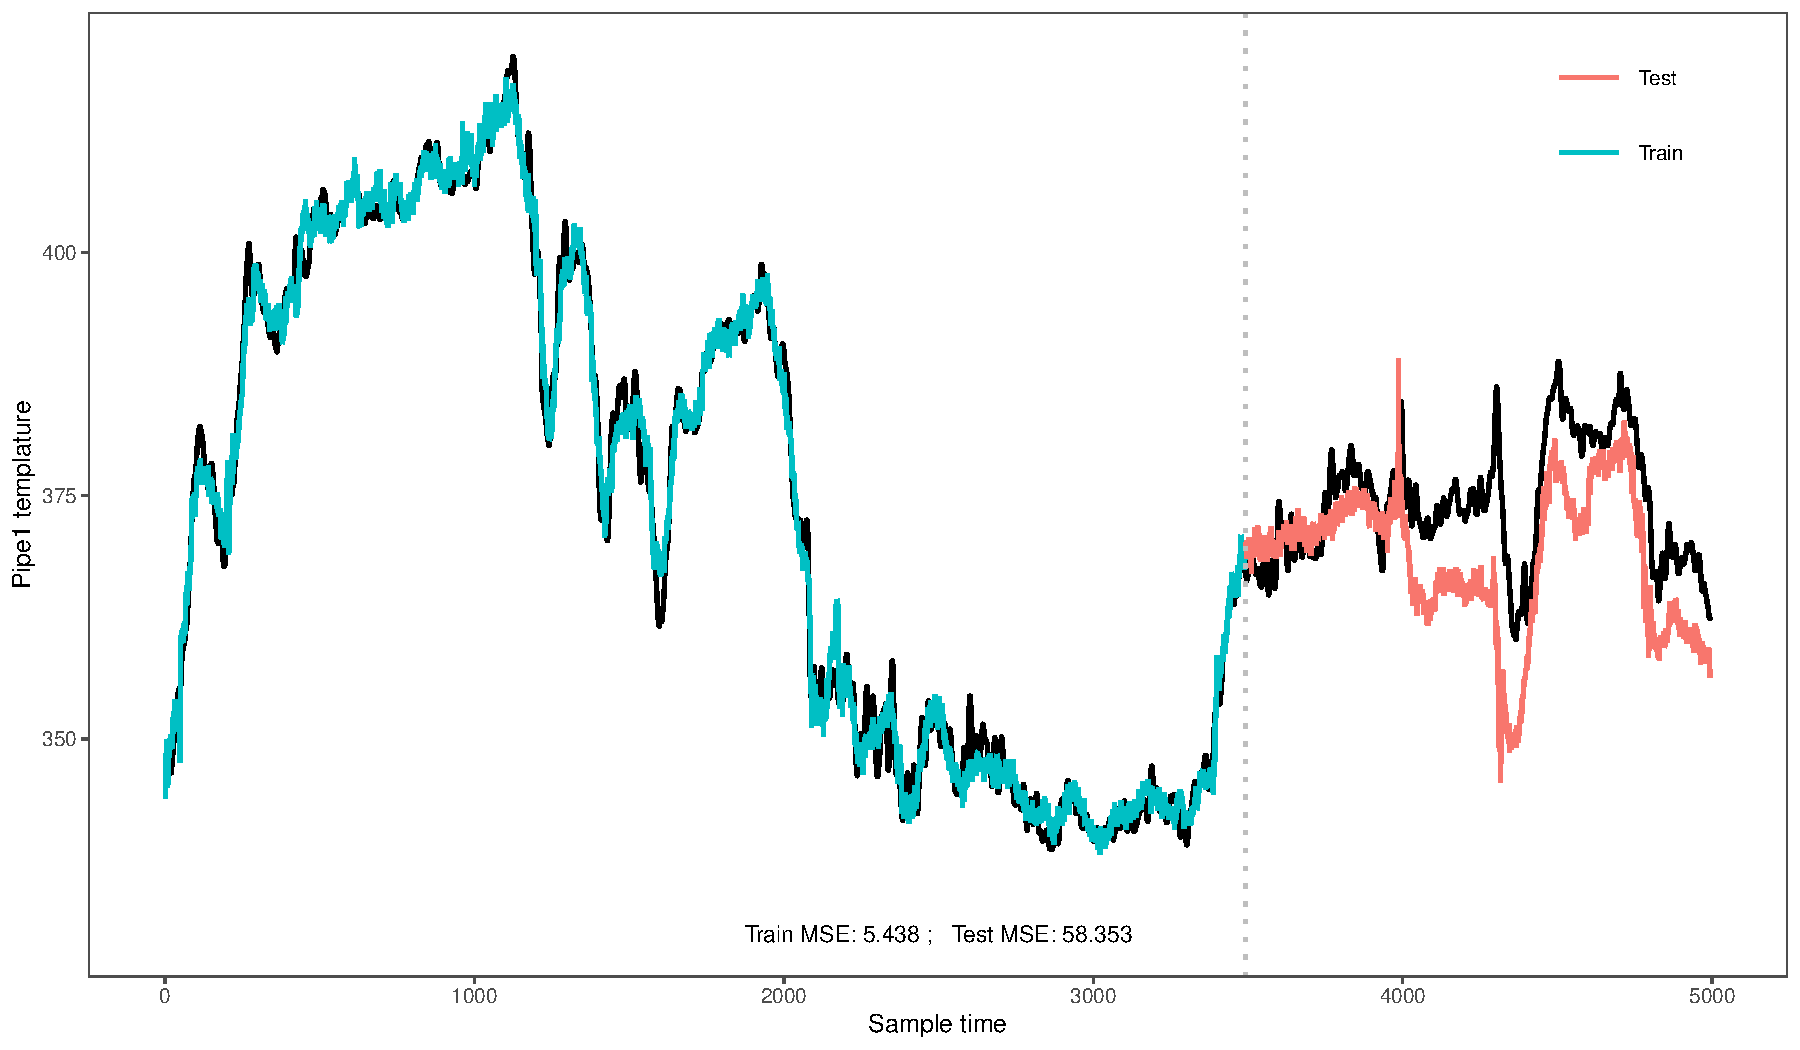
\includegraphics{TJRJCP_DuXingx_202105_files/figure-latex/unnamed-chunk-29-1} 

}

\caption{管道1-Ridge模型拟合效果图}\label{fig:unnamed-chunk-29}
\end{figure}

\begin{figure}

{\centering 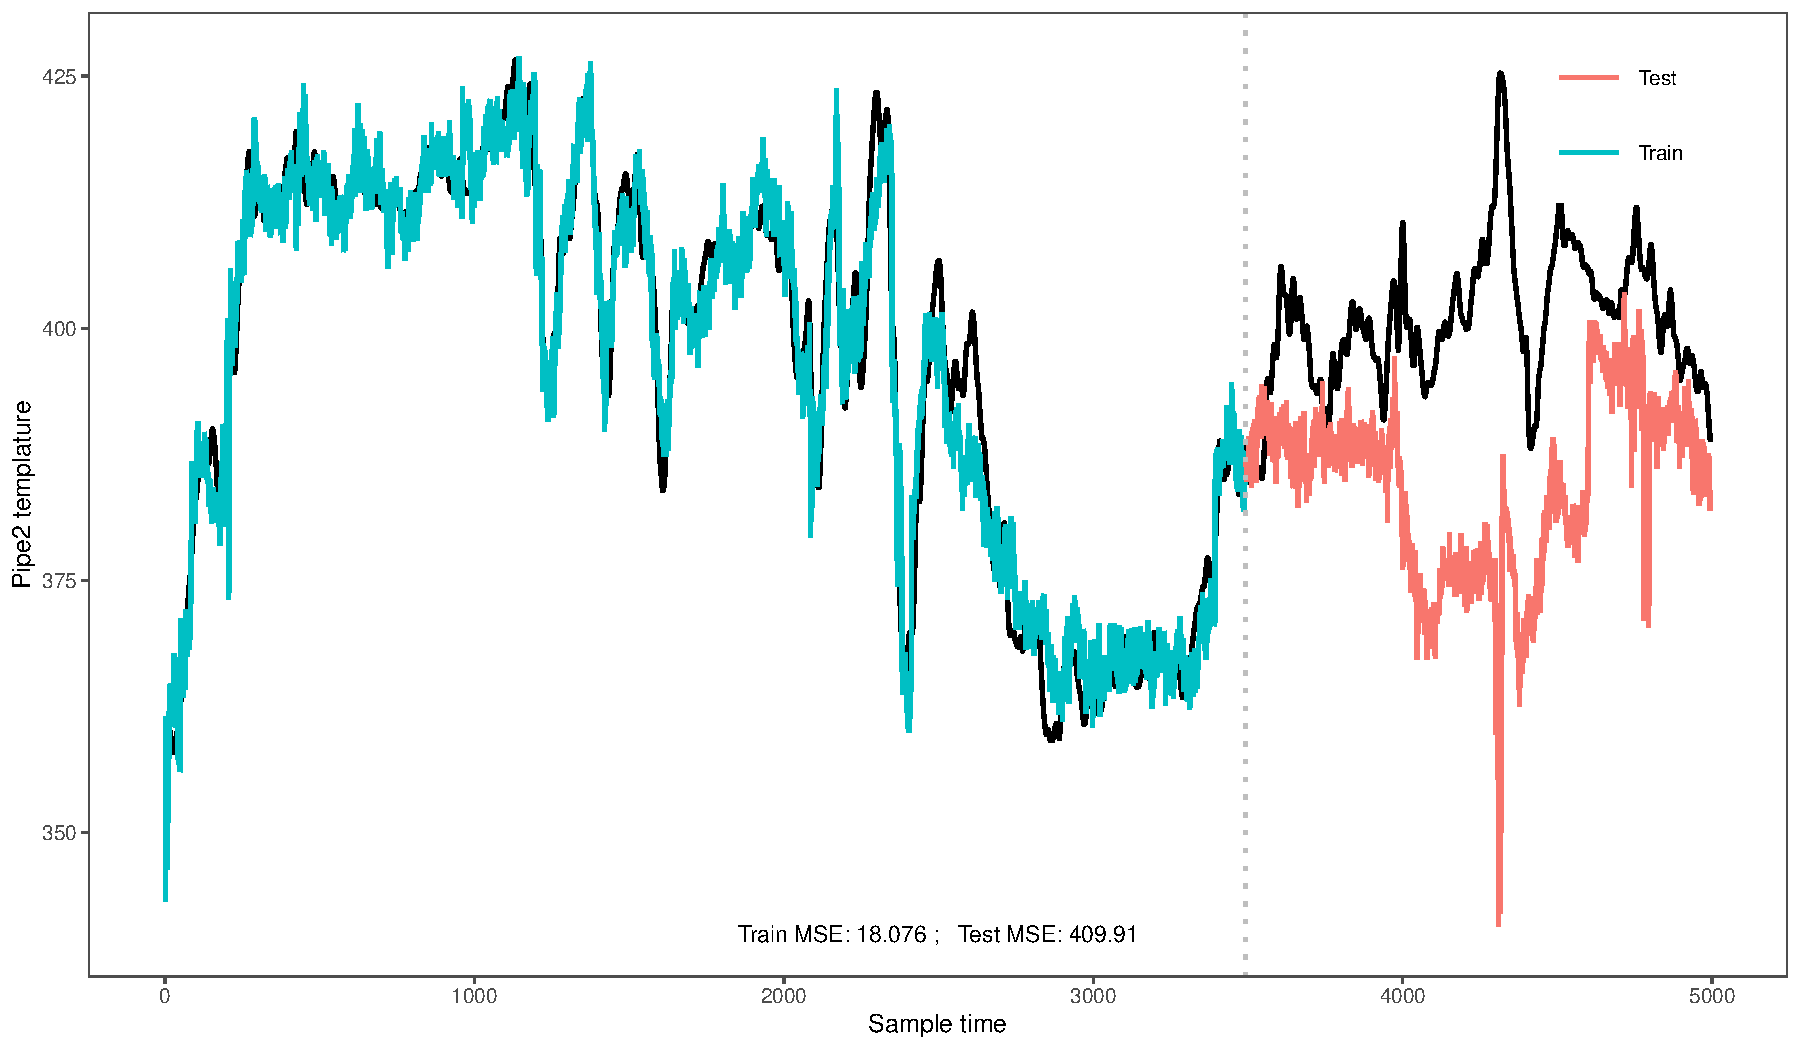
\includegraphics{TJRJCP_DuXingx_202105_files/figure-latex/unnamed-chunk-30-1} 

}

\caption{管道2-Ridge模型拟合效果图}\label{fig:unnamed-chunk-30}
\end{figure}

\begin{figure}

{\centering 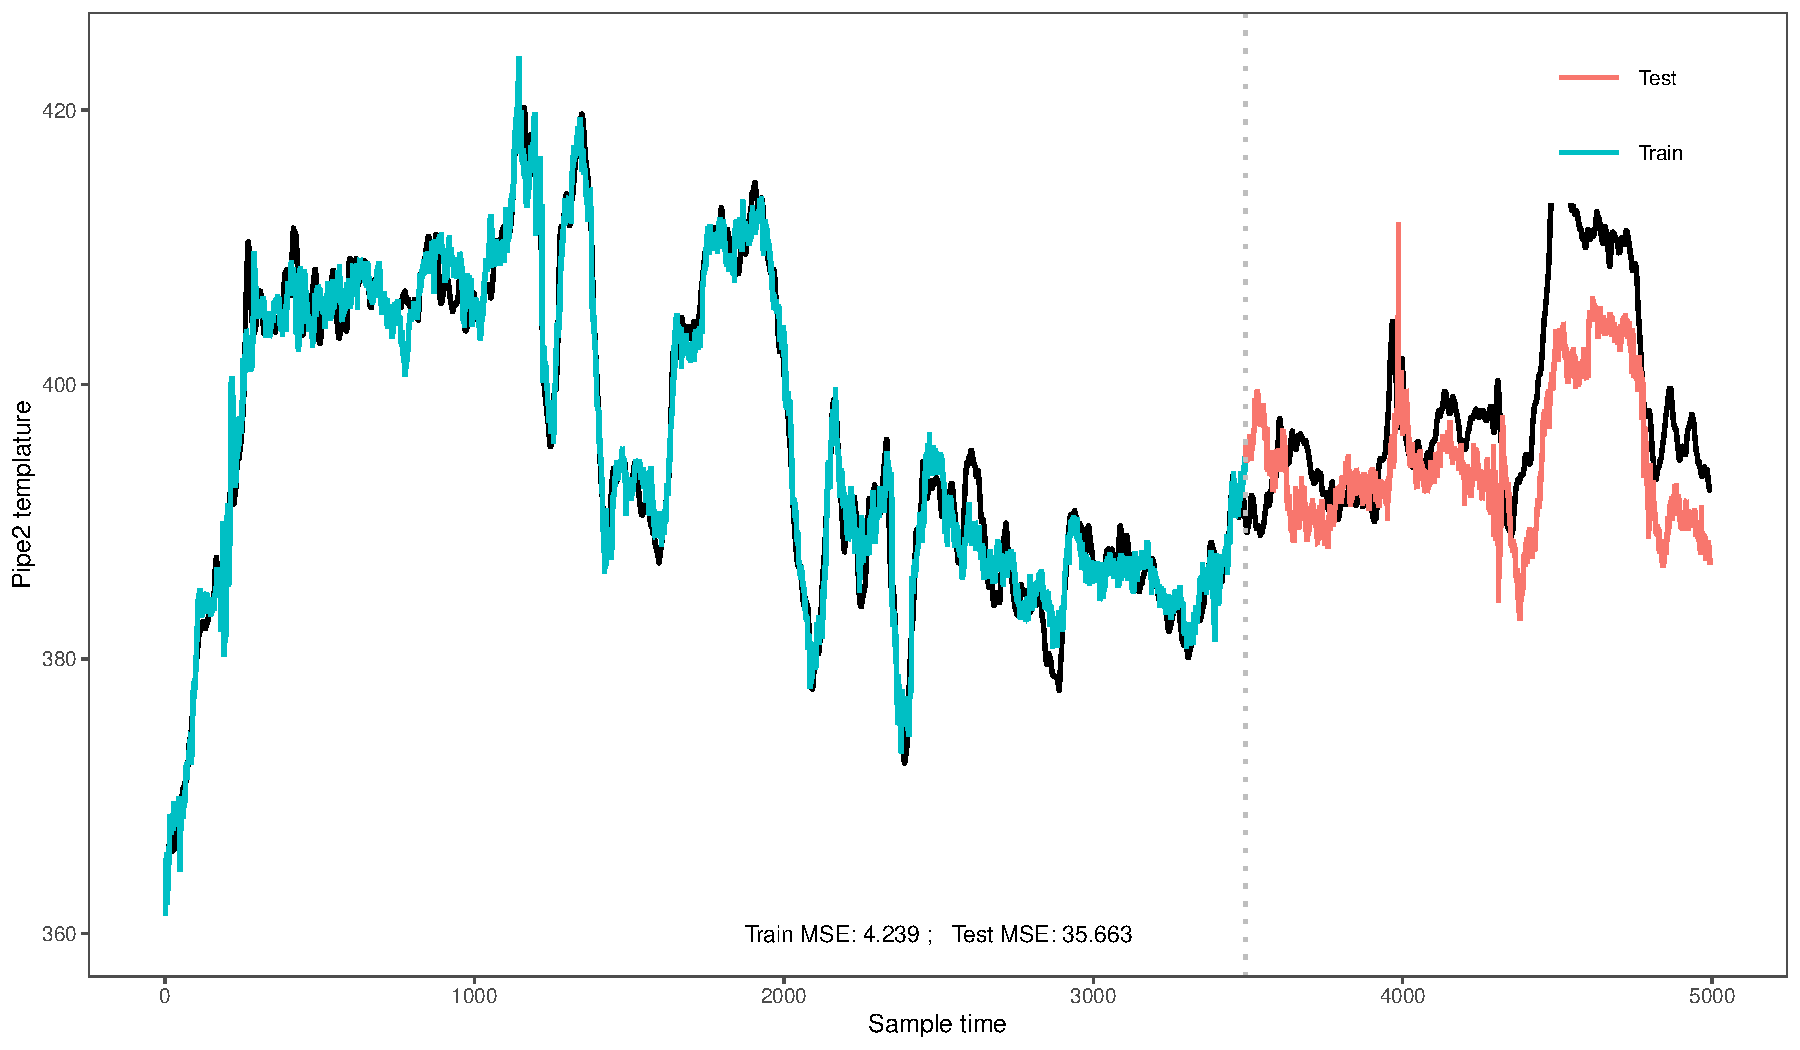
\includegraphics{TJRJCP_DuXingx_202105_files/figure-latex/unnamed-chunk-31-1} 

}

\caption{管道3-Ridge模型拟合效果图}\label{fig:unnamed-chunk-31}
\end{figure}

\begin{figure}

{\centering 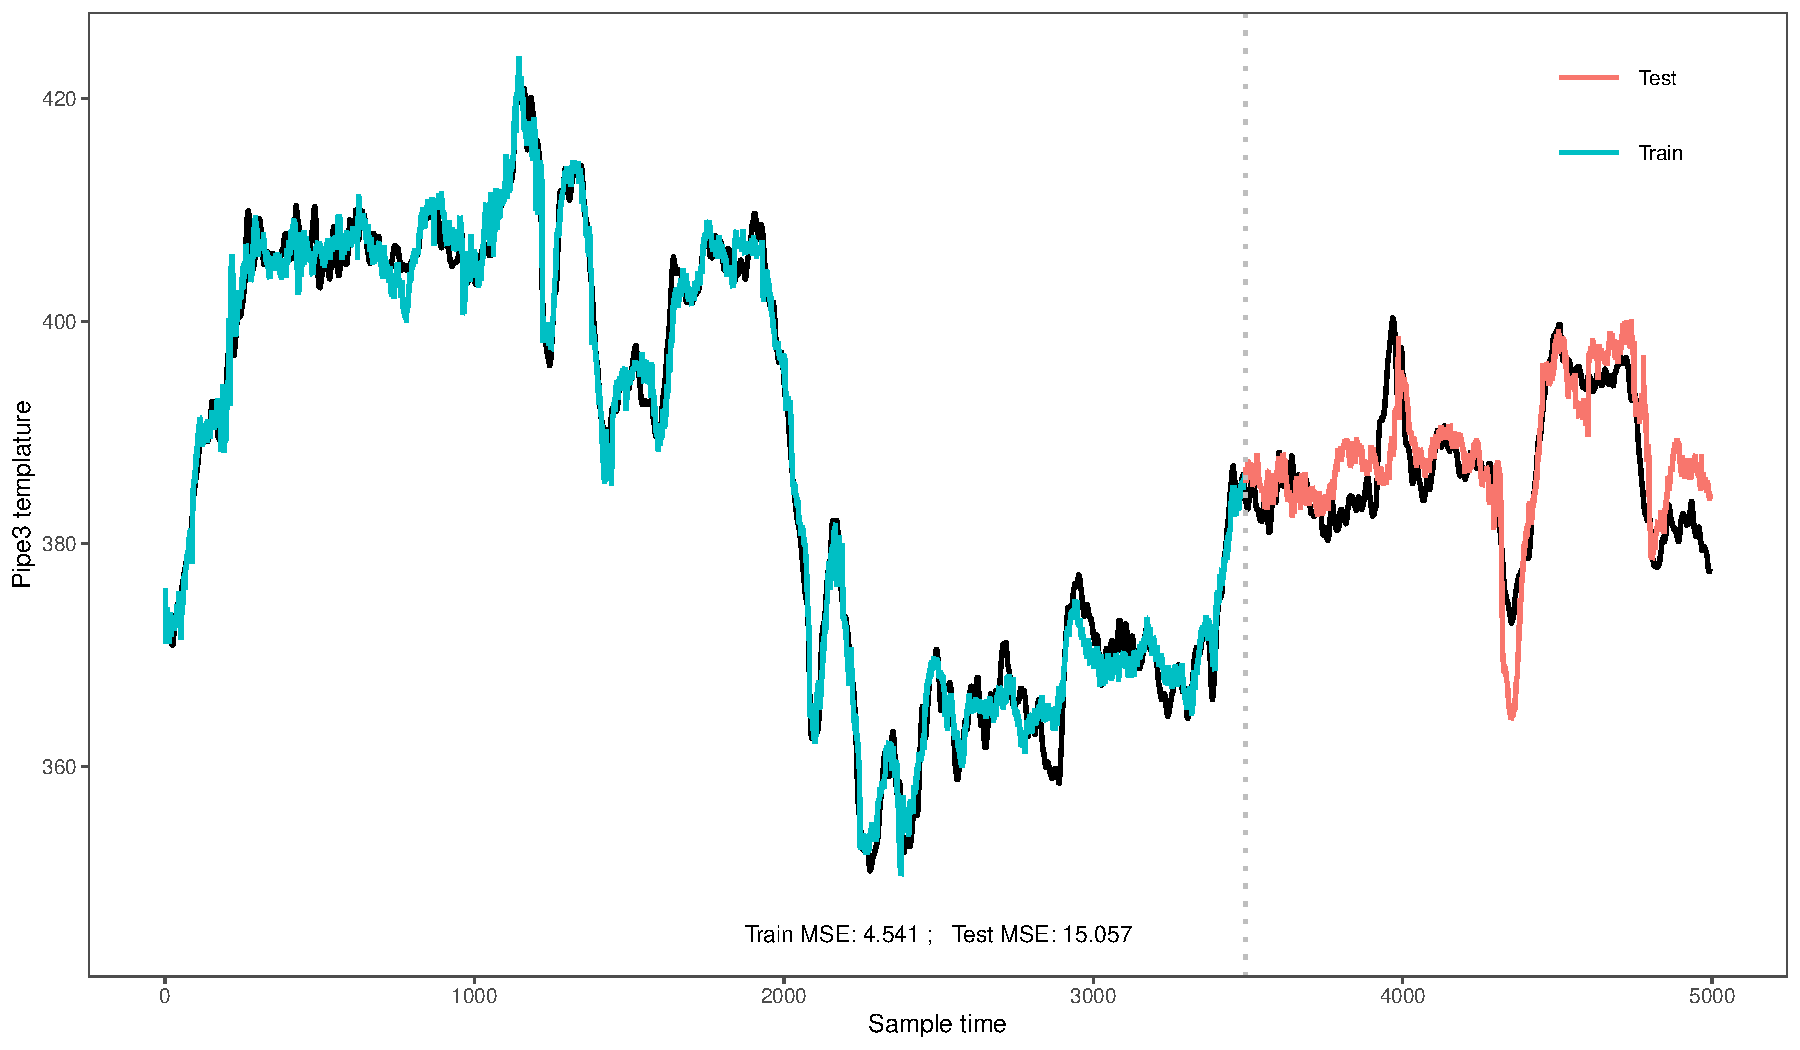
\includegraphics{TJRJCP_DuXingx_202105_files/figure-latex/unnamed-chunk-32-1} 

}

\caption{管道4-Ridge模型拟合效果图}\label{fig:unnamed-chunk-32}
\end{figure}

\begin{figure}

{\centering 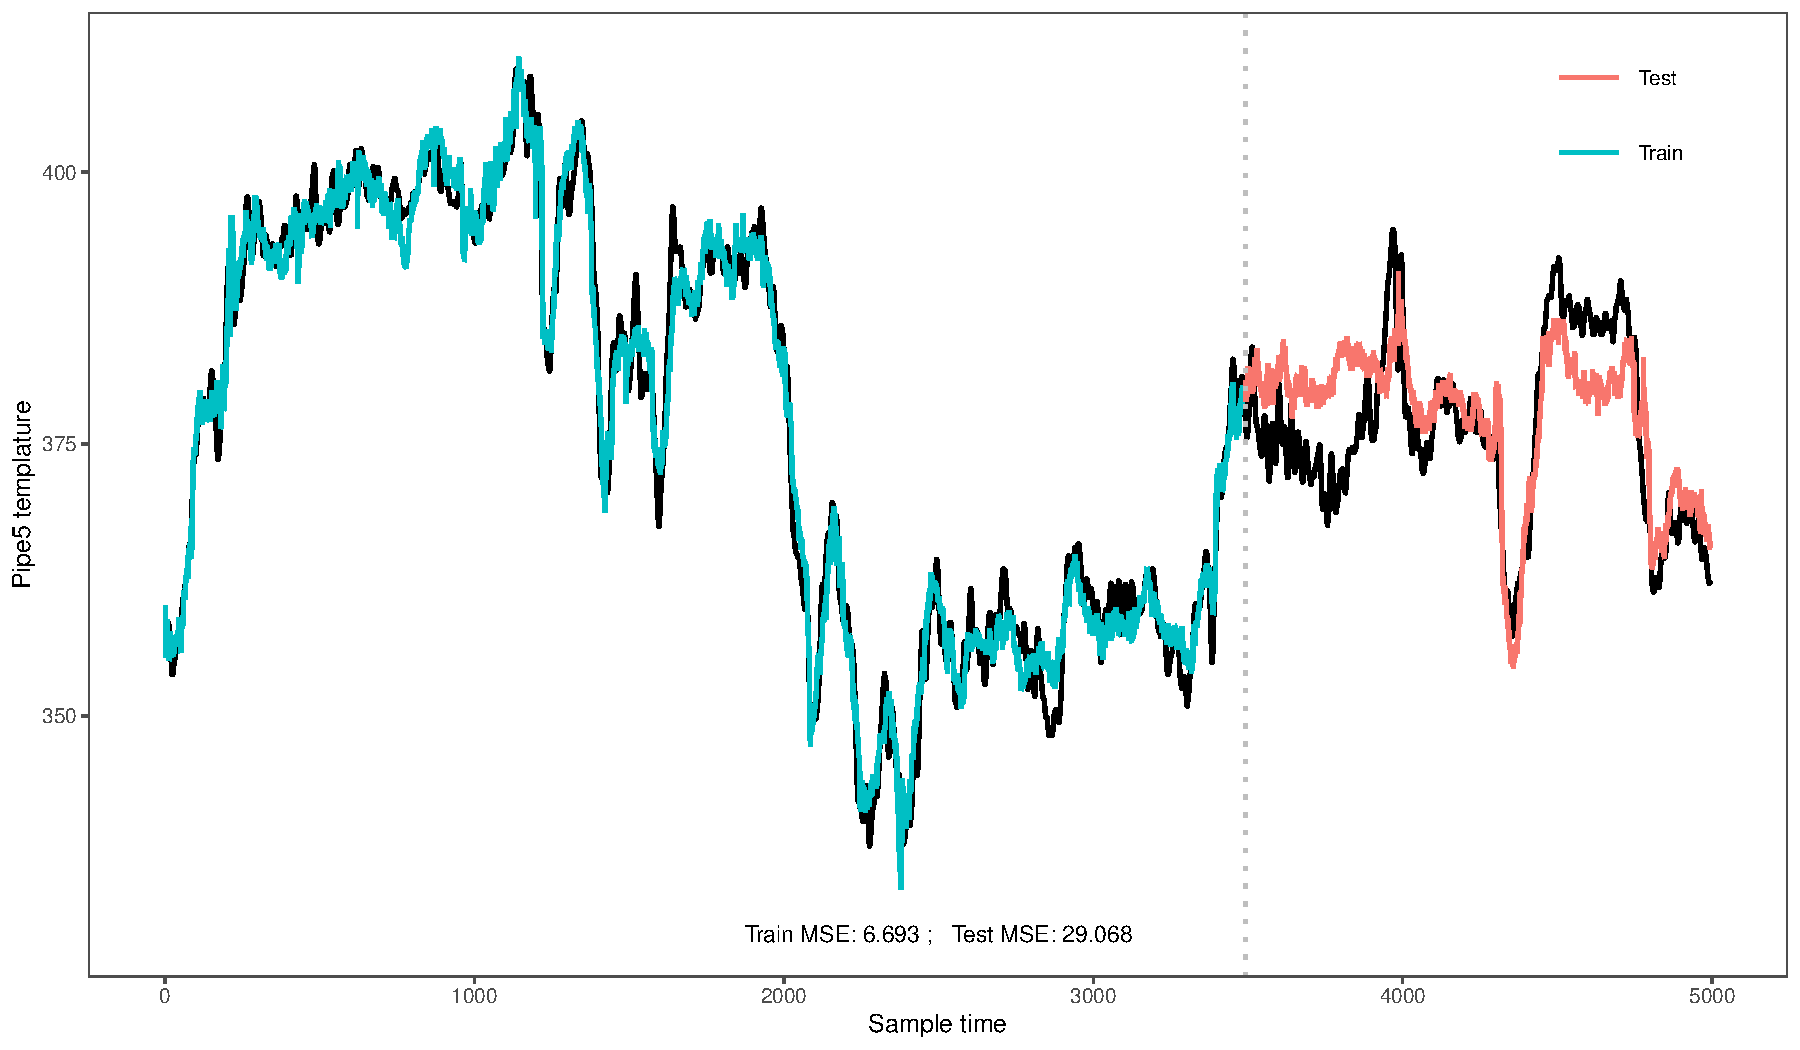
\includegraphics{TJRJCP_DuXingx_202105_files/figure-latex/unnamed-chunk-33-1} 

}

\caption{管道5-Ridge模型拟合效果图}\label{fig:unnamed-chunk-33}
\end{figure}

\begin{figure}

{\centering 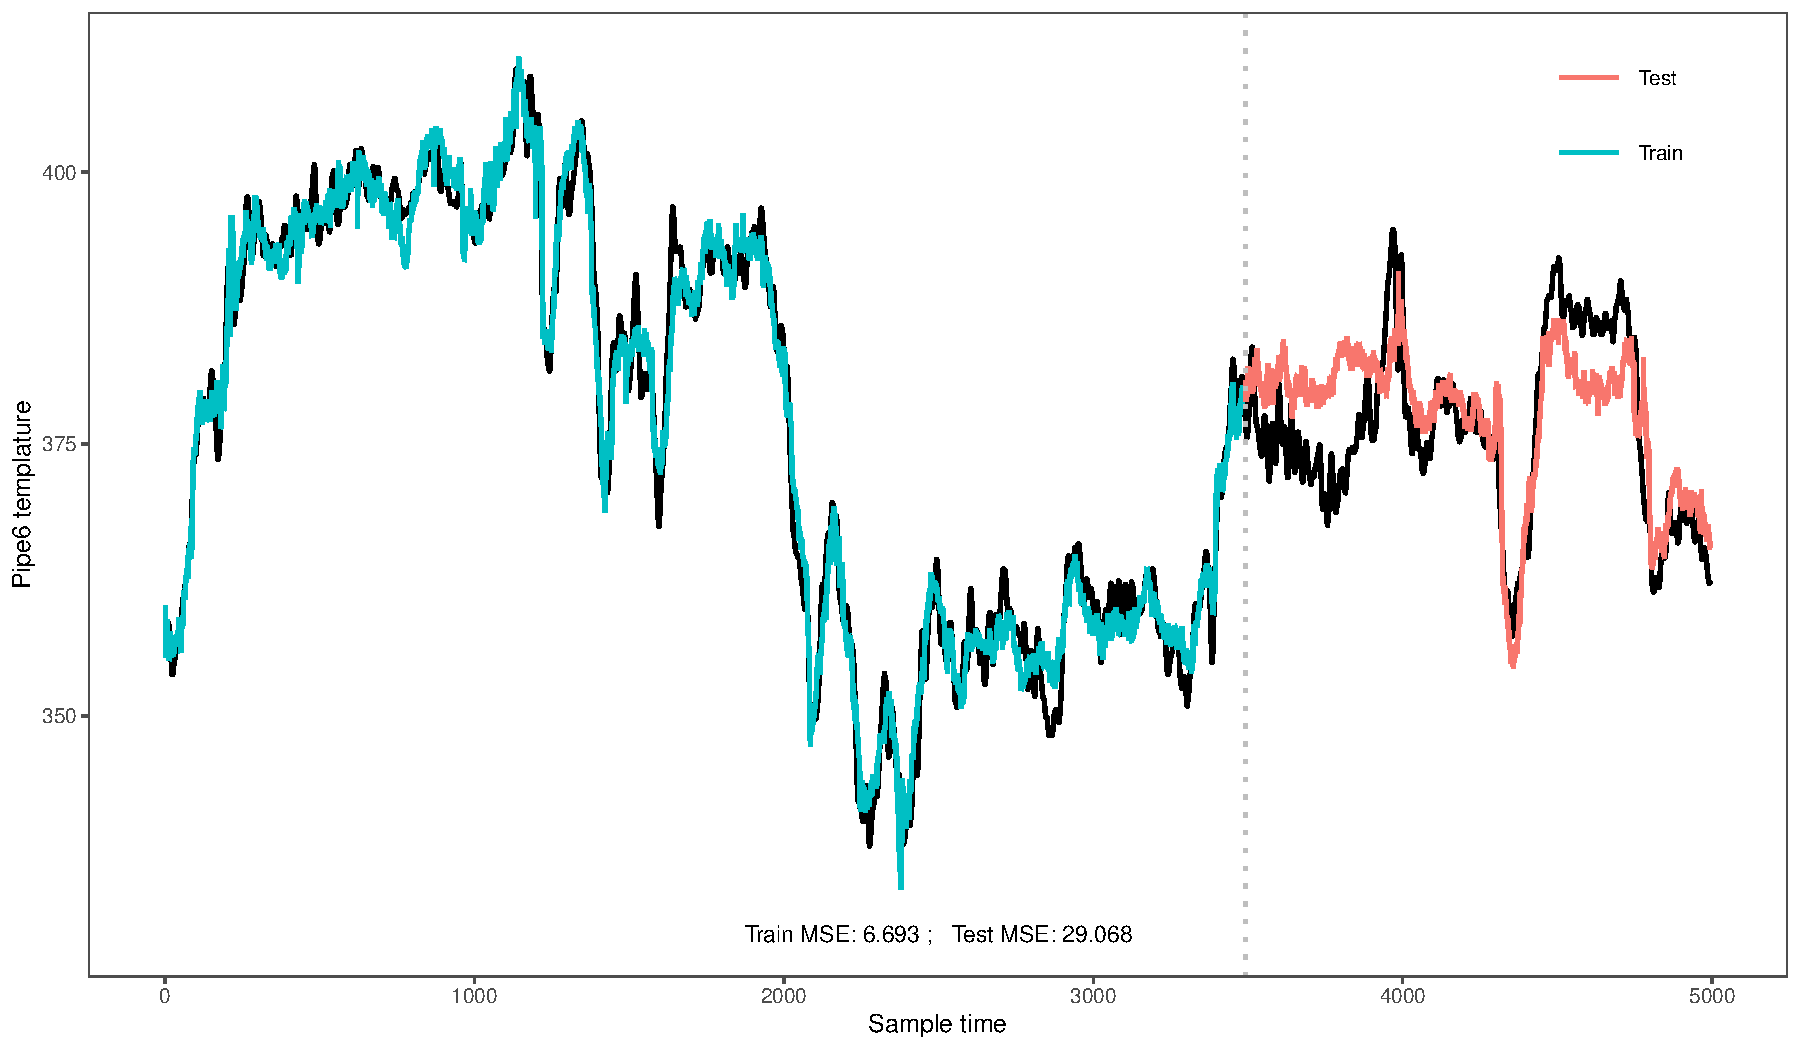
\includegraphics{TJRJCP_DuXingx_202105_files/figure-latex/unnamed-chunk-34-1} 

}

\caption{管道6-Ridge模型拟合效果图}\label{fig:unnamed-chunk-34}
\end{figure}

\begin{figure}

{\centering 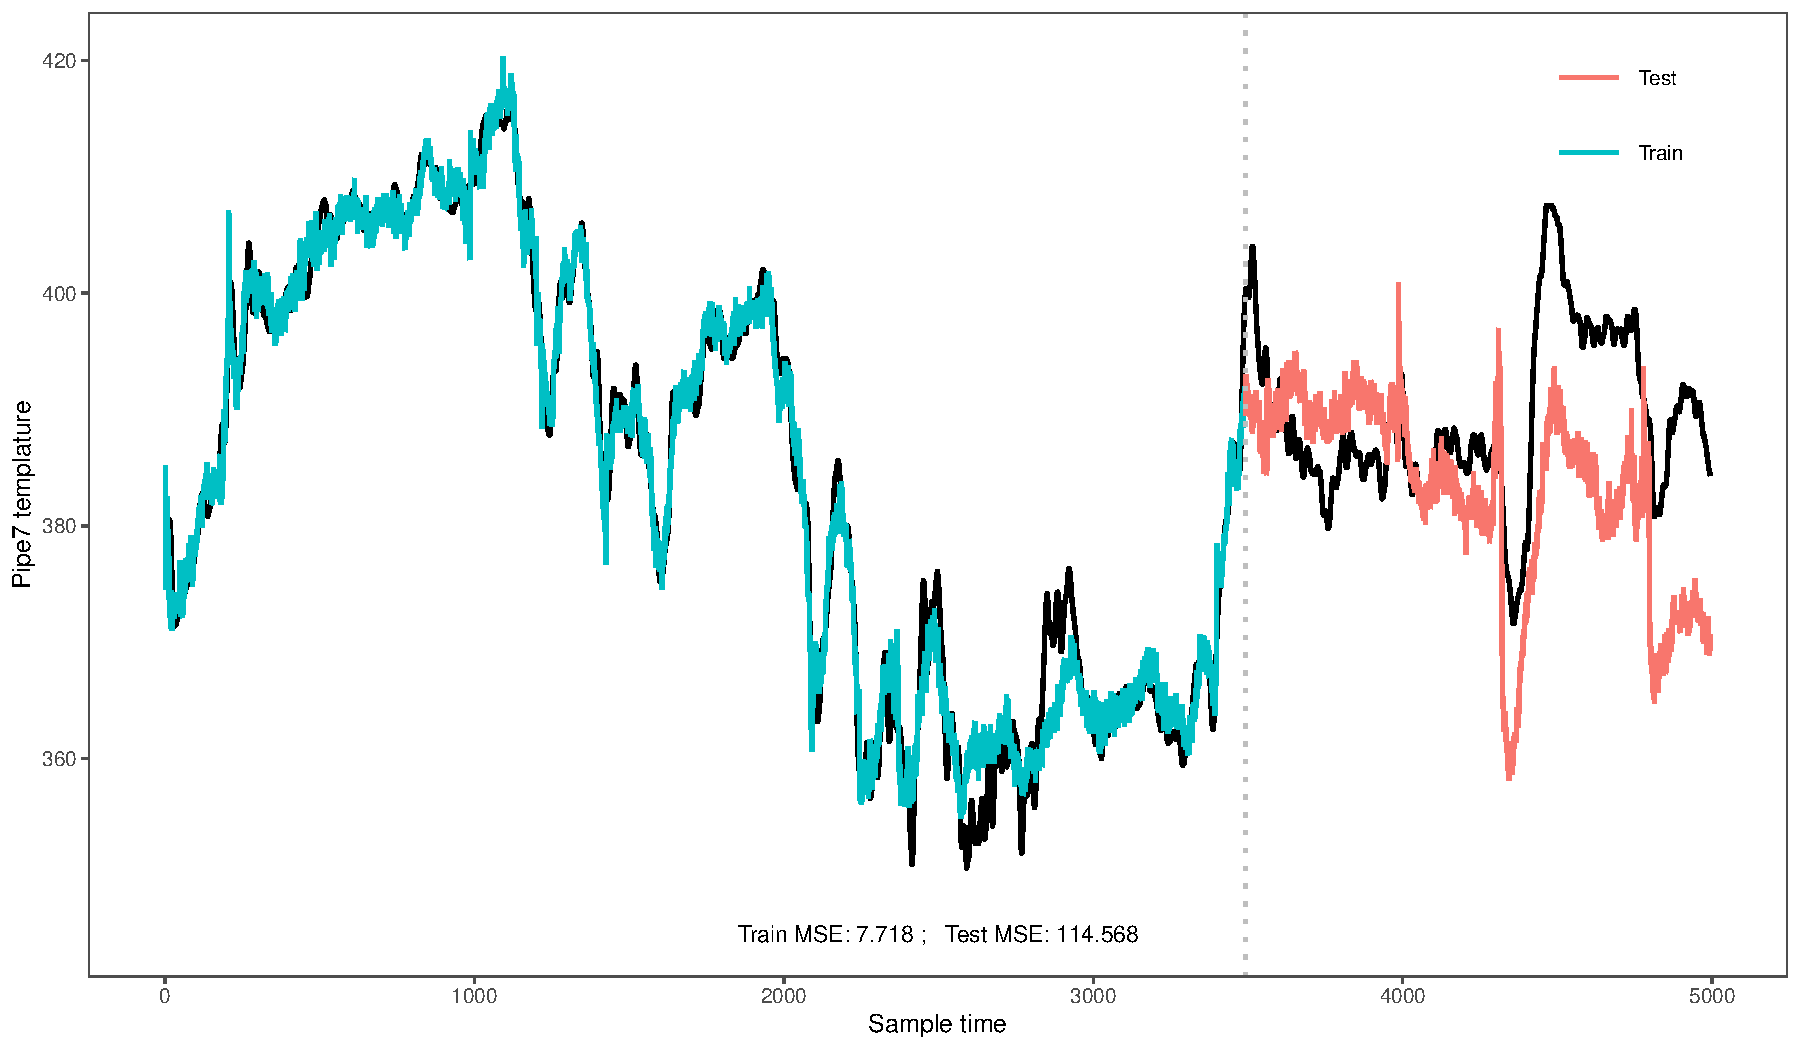
\includegraphics{TJRJCP_DuXingx_202105_files/figure-latex/unnamed-chunk-35-1} 

}

\caption{管道7-Ridge模型拟合效果图}\label{fig:unnamed-chunk-35}
\end{figure}

\begin{figure}

{\centering 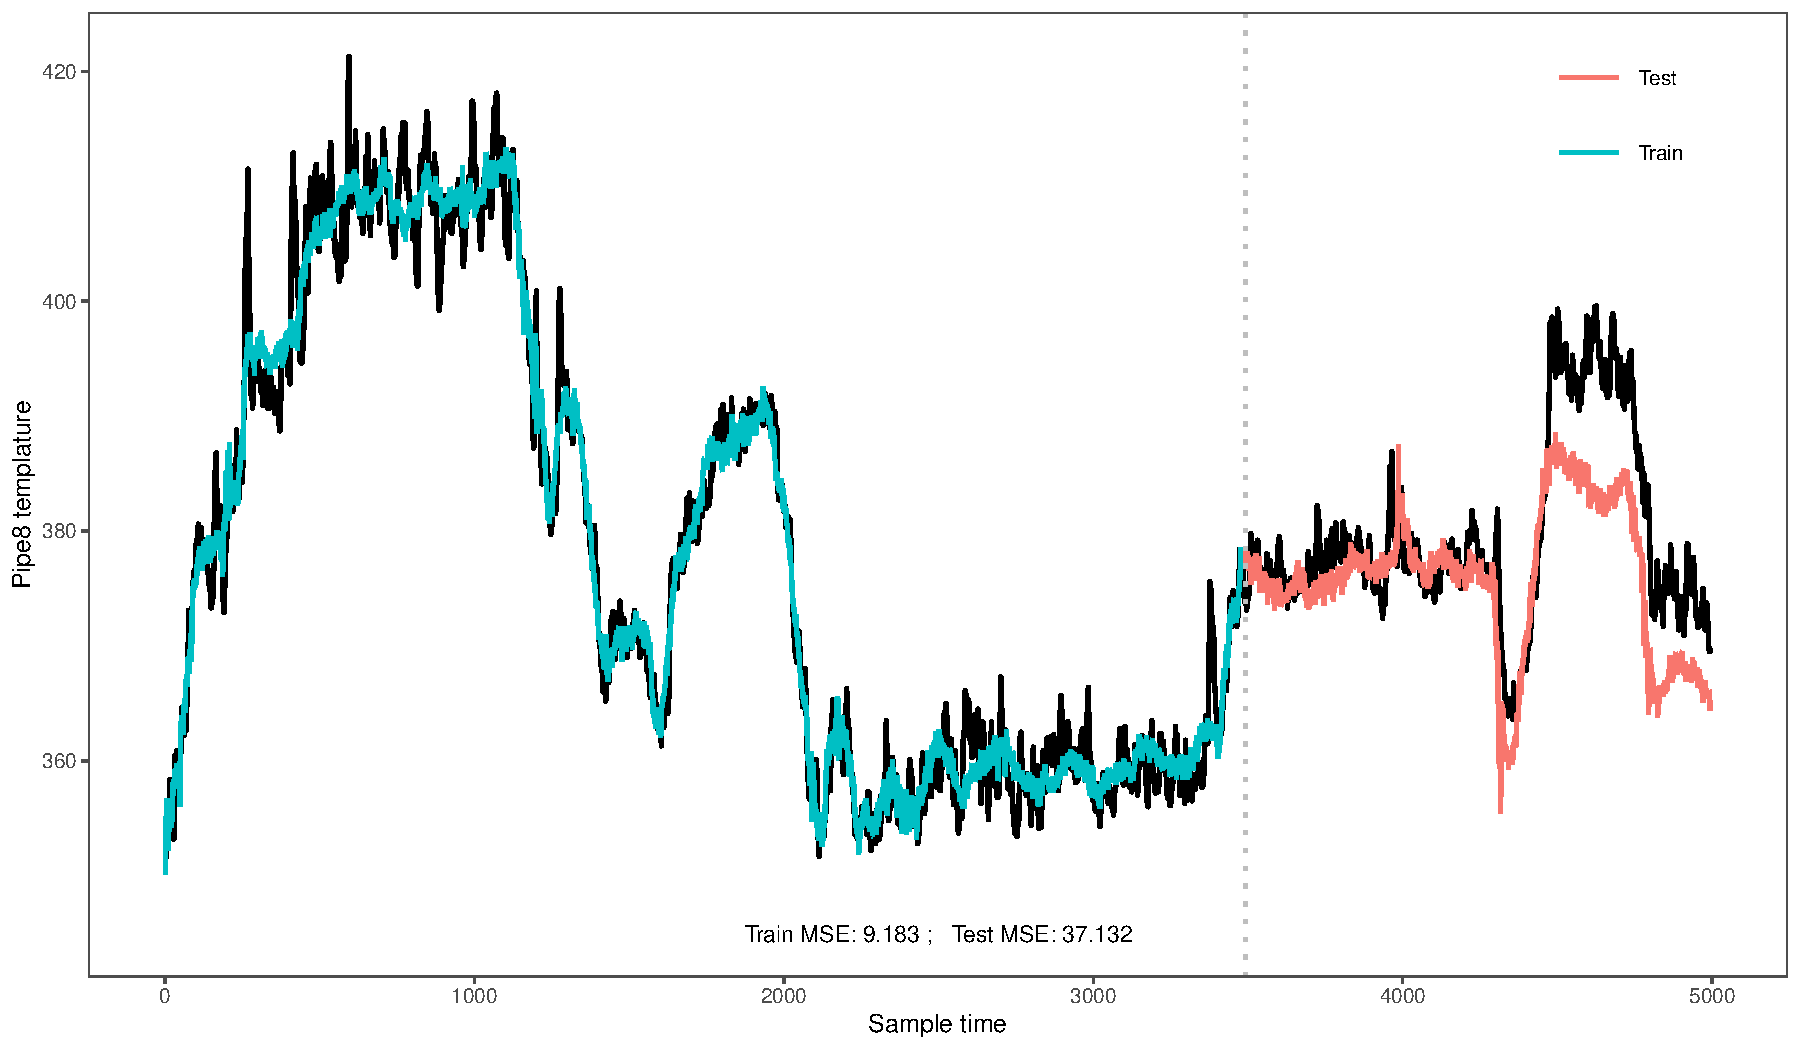
\includegraphics{TJRJCP_DuXingx_202105_files/figure-latex/unnamed-chunk-36-1} 

}

\caption{管道1-Ridge模型拟合效果图}\label{fig:unnamed-chunk-36}
\end{figure}

\begin{figure}

{\centering 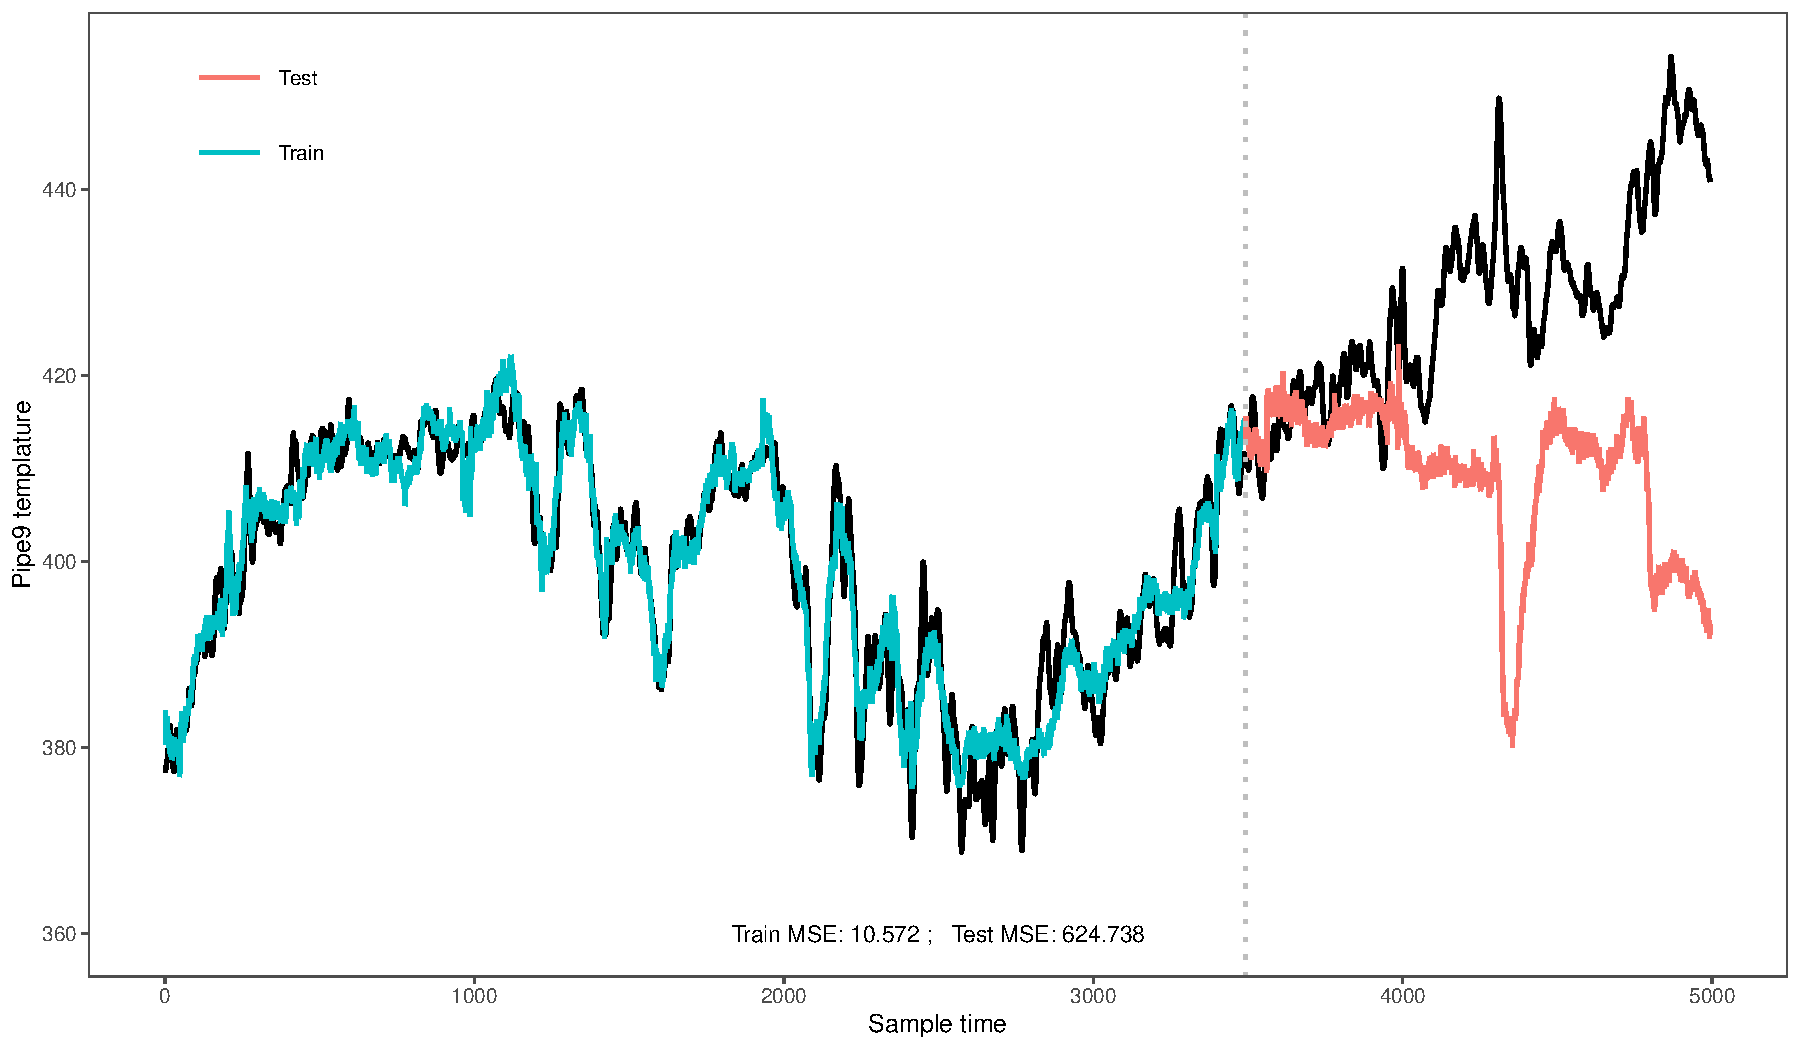
\includegraphics{TJRJCP_DuXingx_202105_files/figure-latex/unnamed-chunk-37-1} 

}

\caption{管道9-Ridge模型拟合效果图}\label{fig:unnamed-chunk-37}
\end{figure}

\begin{figure}

{\centering 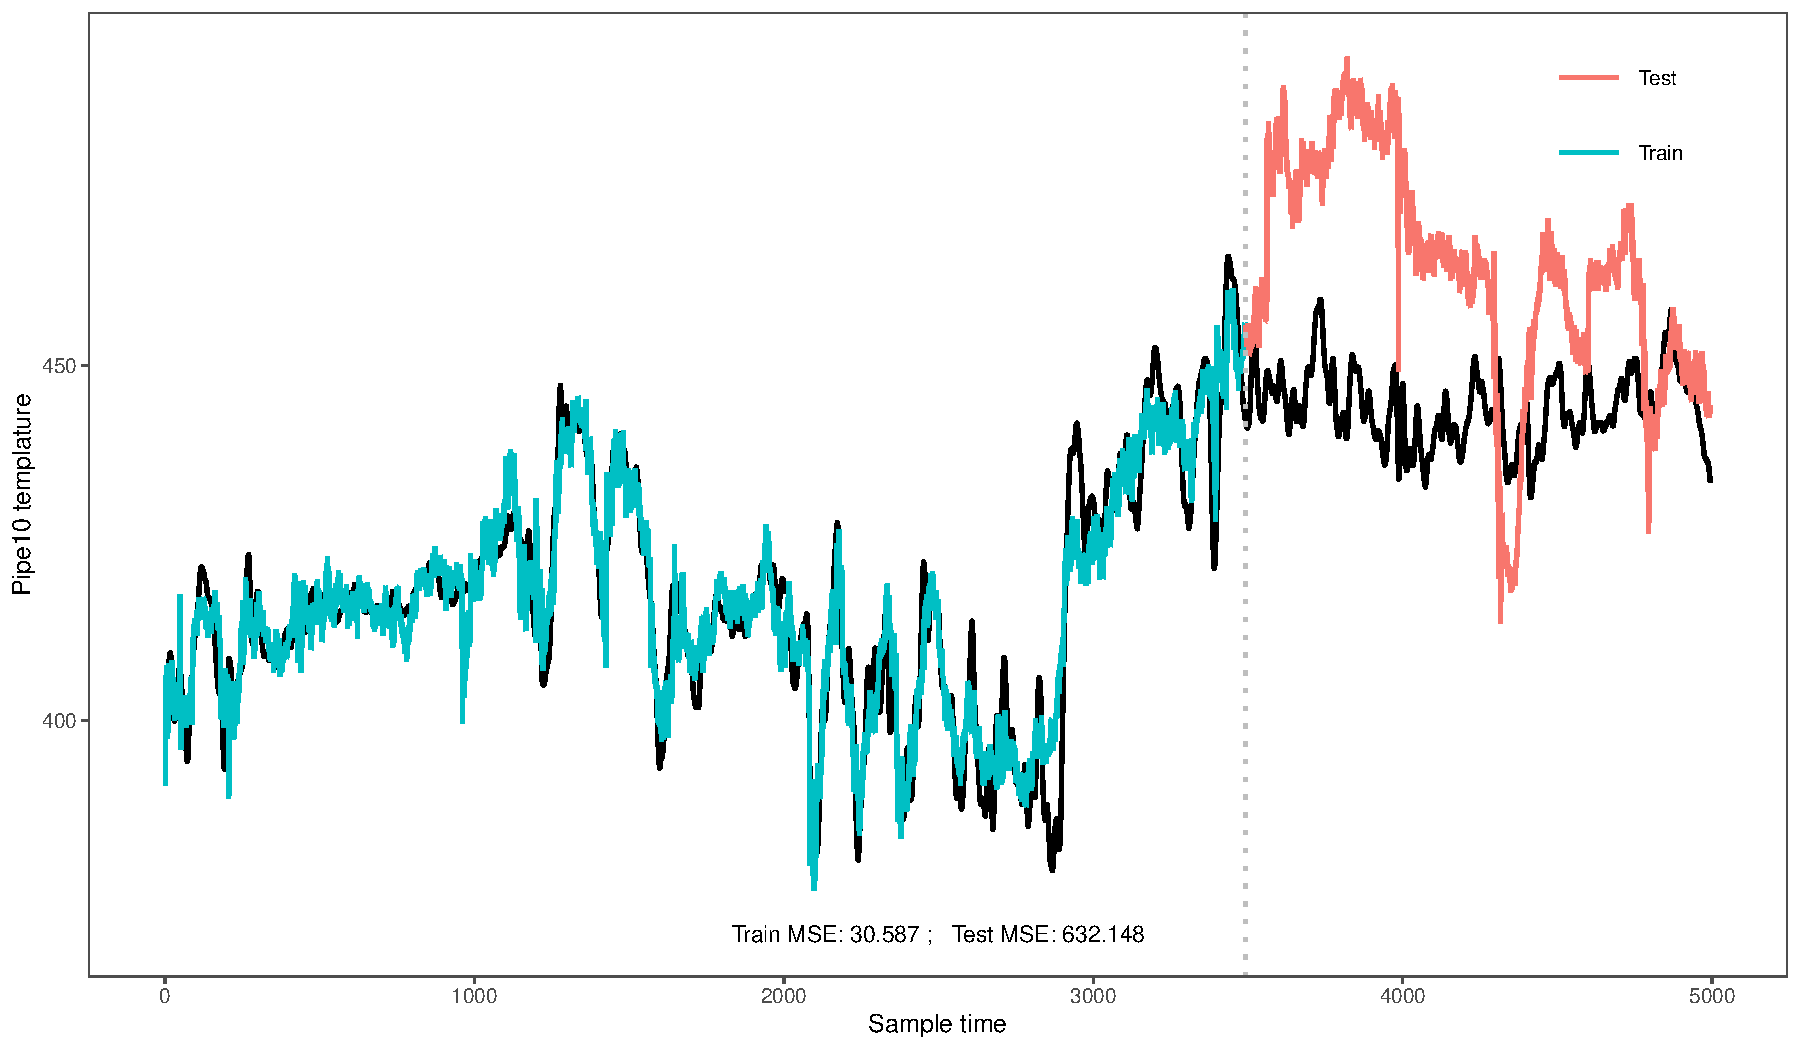
\includegraphics{TJRJCP_DuXingx_202105_files/figure-latex/unnamed-chunk-38-1} 

}

\caption{管道10-Ridge模型拟合效果图}\label{fig:unnamed-chunk-38}
\end{figure}

\end{document}
